% This is "sig-alternate.tex" V2.1 April 2013
% This file should be compiled with V2.5 of "sig-alternate.cls" May 2012
%
% This example file demonstrates the use of the 'sig-alternate.cls'
% V2.5 LaTeX2e document class file. It is for those submitting
% articles to ACM Conference Proceedings WHO DO NOT WISH TO
% STRICTLY ADHERE TO THE SIGS (PUBS-BOARD-ENDORSED) STYLE.
% The 'sig-alternate.cls' file will produce a similar-looking,
% albeit, 'tighter' paper resulting in, invariably, fewer pages.
%
% ----------------------------------------------------------------------------------------------------------------
% This .tex file (and associated .cls V2.5) produces:
%       1) The Permission Statement
%       2) The Conference (location) Info information
%       3) The Copyright Line with ACM data
%       4) NO page numbers
%
% as against the acm_proc_article-sp.cls file which
% DOES NOT produce 1) thru' 3) above.
%
% Using 'sig-alternate.cls' you have control, however, from within
% the source .tex file, over both the CopyrightYear
% (defaulted to 200X) and the ACM Copyright Data
% (defaulted to X-XXXXX-XX-X/XX/XX).
% e.g.
% \CopyrightYear{2007} will cause 2007 to appear in the copyright line.
% \crdata{0-12345-67-8/90/12} will cause 0-12345-67-8/90/12 to appear in the copyright line.
%
% ---------------------------------------------------------------------------------------------------------------
% This .tex source is an example which *does* use
% the .bib file (from which the .bbl file % is produced).
% REMEMBER HOWEVER: After having produced the .bbl file,
% and prior to final submission, you *NEED* to 'insert'
% your .bbl file into your source .tex file so as to provide
% ONE 'self-contained' source file.
%
% ================= IF YOU HAVE QUESTIONS =======================
% Questions regarding the SIGS styles, SIGS policies and
% procedures, Conferences etc. should be sent to
% Adrienne Griscti (griscti@acm.org)
%
% Technical questions _only_ to
% Gerald Murray (murray@hq.acm.org)
% ===============================================================

\documentclass{sig-alternate}

\usepackage{mathtools}
\usepackage[urlbordercolor={1 1 1},citebordercolor={1 1 1},linkbordercolor={1 1 1}]{hyperref}
\usepackage{enumitem}
\usepackage{tikz}
\usetikzlibrary{decorations.text}
\usepackage{tkz-berge}

% https://tex.stackexchange.com/questions/42271/floor-and-ceiling-functions
\DeclarePairedDelimiter{\ceil}{\lceil}{\rceil}
\DeclarePairedDelimiter{\floor}{\lfloor}{\rfloor}

\newcommand*\concat{\mathbin{\|}}

\begin{document}

% Copyright
\setcopyright{acmcopyright}
%\setcopyright{acmlicensed}
%\setcopyright{rightsretained}
%\setcopyright{usgov}
%\setcopyright{usgovmixed}
%\setcopyright{cagov}
%\setcopyright{cagovmixed}

% DOI
\doi{10.475/123_4}

% ISBN
\isbn{123-4567-24-567/08/06}

%Conference
\conferenceinfo{ACM CCS '14}{October 12-16, 2015, Denver, Colorado, USA}

\acmPrice{\$15.00}

% --- Author Metadata here ---
%\conferenceinfo{WOODSTOCK}{'97 El Paso, Texas USA}
\CopyrightYear{2015} % Allows default copyright year (20XX) to be over-ridden - IF NEED BE.
%\crdata{0-12345-67-8/90/01}  % Allows default copyright data (0-89791-88-6/97/05) to be over-ridden - IF NEED BE.
% --- End of Author Metadata ---

\title{The Onion Name System}
\subtitle{Tor-powered Distributed DNS for Tor Hidden Services}

\numberofauthors{2}
\author{
% 1st. author
\alignauthor
Jesse Victors \\
       \affaddr{7449 S. Babcock Blvd.}\\
       \affaddr{Wasilla, AK 99623}\\
       \email{jvictors@jessevictors.com}
% 2nd. author
\alignauthor
Ming Li\\
       \affaddr{Utah State University}\\
       \affaddr{Logan, UT 84321}\\
       \email{ming.li@usu.edu}
}

\maketitle

\begin{abstract} % done

Tor is a third-generation low-latency onion router that provides its users with online privacy, anonymity, and resistance to traffic analysis. In recent years its userbase, network, and community has grown significantly in response to revelations of international electronic surveillance, and it remains one of the most popular anonymity networks in use today. Tor also provides access to anonymous servers known as hidden services -- servers of unknown location and ownership who achieve anonymity through Tor circuits. These hidden services can be accessed through any Tor-enabled web browser but they suffer from usability challenges due to the algorithmic generation of their addresses.

In response to this difficulty, in this work we introduce the Onion Name System (OnioNS), a privacy-enhanced distributed DNS that allows users to reference a hidden service by a meaningful globally-unique self-authenticating domain name chosen by the hidden service operator. We introduce a new distributed self-healing database and construct OnioNS as an optional backwards-compatible plugin for Tor on top of existing hidden service infrastructure. We simplify our design and threat model by embedding OnioNS within the Tor network and provide mechanisms for authenticated denial-of-existence with minimal networking costs. Our reference implementation demonstrates that OnioNS successfully addresses the major usability issue that has been with Tor hidden services since their introduction in 2002.

\end{abstract}

% http://dl.acm.org/ccs.cfm
% http://www.acm.org/about/class/
% https://academia.stackexchange.com/questions/15252/is-the-new-acm-2012-taxonomy-usable-in-use
\begin{CCSXML}
<ccs2012>
<concept>
<concept_id>10002951.10003152.10003161.10003164</concept_id>
<concept_desc>Information systems~Block / page strategies</concept_desc>
<concept_significance>500</concept_significance>
</concept>
<concept>
<concept_id>10003033.10003099.10003037</concept_id>
<concept_desc>Networks~Naming and addressing</concept_desc>
<concept_significance>500</concept_significance>
</concept>
<concept>
<concept_id>10002978.10003006.10003013</concept_id>
<concept_desc>Security and privacy~Distributed systems security</concept_desc>
<concept_significance>300</concept_significance>
</concept>
<concept>
<concept_id>10002978.10002979</concept_id>
<concept_desc>Security and privacy~Cryptography</concept_desc>
<concept_significance>100</concept_significance>
</concept>
<concept>
<concept_id>10002978.10003014.10003015</concept_id>
<concept_desc>Security and privacy~Security protocols</concept_desc>
<concept_significance>100</concept_significance>
</concept>
</ccs2012>
\end{CCSXML}

\ccsdesc[500]{Information systems~Block / page strategies}
\ccsdesc[500]{Networks~Naming and addressing}
\ccsdesc[300]{Security and privacy~Distributed systems security}
\ccsdesc[100]{Security and privacy~Cryptography}
\ccsdesc[100]{Security and privacy~Security protocols}

%{Security and privacy}
%	Cryptography
%	Systems security
%		Distributed systems security
%	 Network security
%	 	Security protocols
%{Information systems}
%	{Information storage systems}
%		Record storage systems
%			Block / page strategies
%{Networks}
%	Network services
%		Naming and addressing

\printccsdesc

\keywords{Tor, onion, hidden service, anonymity, privacy, network security, petname}

\section{Introduction} % done

As the prevalence of the Internet and other communication has grown, so too has the development and usage of privacy-enhancing systems. These are protocols that provide privacy by obfuscating the link between a user's identity or location and their communications. Privacy is not achieved in traditional Internet connections because SSL/TLS encryption cannot hide IP and TCP headers, which must be exposed to allow routing between two parties; eavesdroppers can easily break user privacy by monitoring these headers.\cite{miller2014know} Following a general distrust of unsecured Internet communications and in light of the 2013-current revelations by Edward Snowden of international Internet mass-surveillance, users have increasingly turned to these tools for their own protection.

Today, most anonymity tools descend from mixnets. Mixnets have inspired the development of many varied mixnet-like protocols and have generated significant literature within the field of network security.\cite{edman2009anonymity} Mixnet descendants can generally be classified into two distinct categories: high-latency and low-latency systems. High-latency networks typically delay traffic packets, increasing their resistance to global adversaries who monitor communication entering and exiting the network. By contrast, low-latency networks do not delay packets and are thus better suited for common Internet activities such as web browsing, instant messaging, or the prompt transmission of email.\cite{dingledine2004tor} In this work, we detail and introduce new functionality within low-latency protocols.

\begin{figure}[htbp]
	\centering
	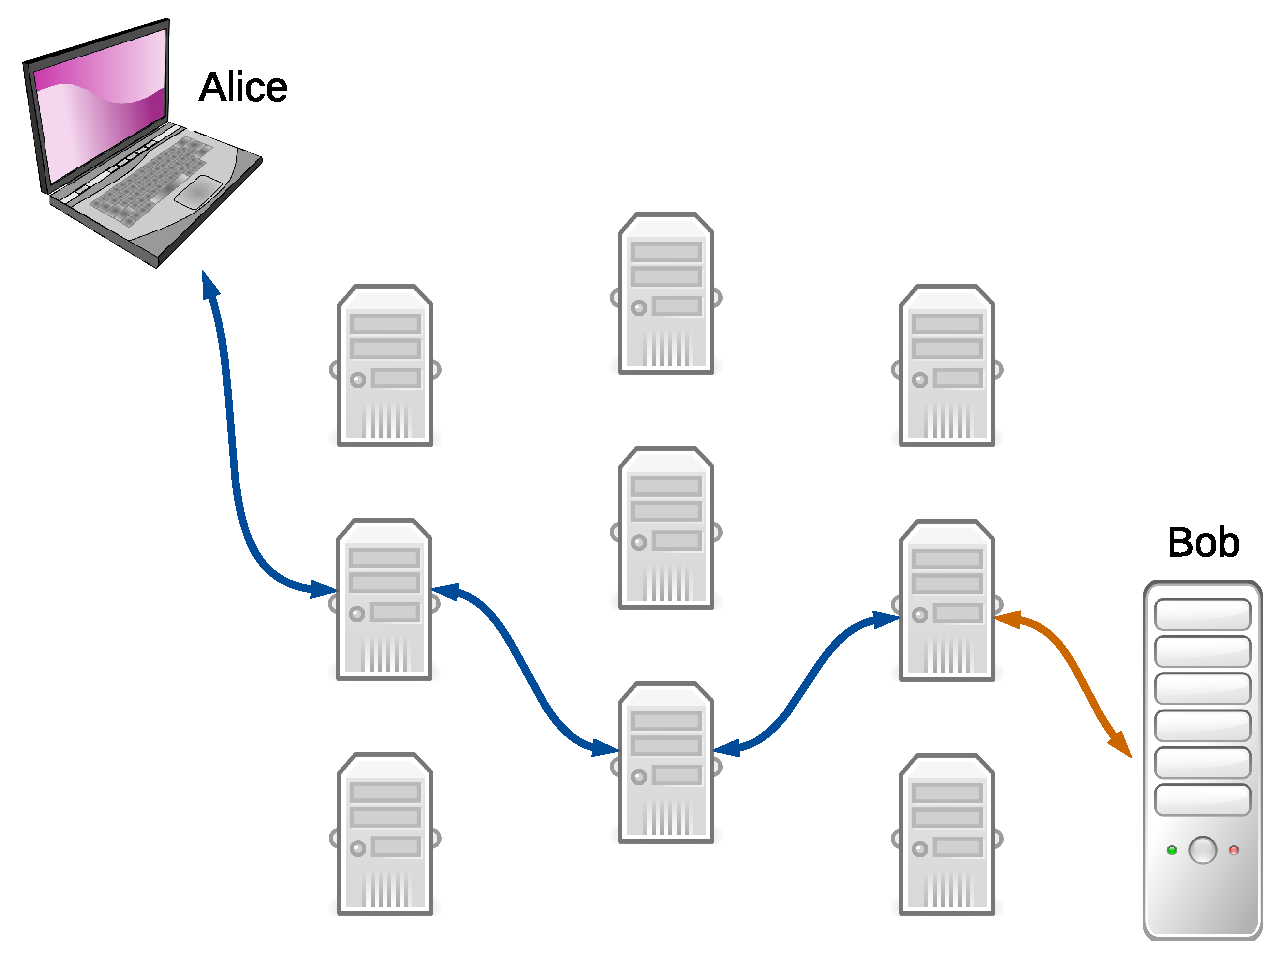
\includegraphics[width=0.4\textwidth]{../images/LucidCharts/Tor_Circuit.pdf}
	\caption{Alice communicates privately to Bob through a Tor circuit. Her communication path consists of three routers, an entry, middle, and exit. Each encrypted Tor link is shown in blue, the final connection from the exit to Bob, shown in orange, is optionally encrypted.}
\end{figure}

Onion routing is the most popular low-latency descendant of mixnets in use today. In onion routing, a user selects a set (typically three) of network nodes, typically called \emph{onion routers} and together a \emph{circuit}, and encrypts the message with the public key of each router. Each encryption layer contains the next destination for the message -- the last layer contains the message's final destination. As the \emph{cell} containing the message travels through the network, each of these onion routers in turn decrypt their encryption layer, exposing their share of the routing information. The final recipient receives the message from the last router, but is never exposed to the message's source. The sender therefore has privacy because the recipient does not know the sender's location, and the sender has anonymity if no identifiable or distinguishing information is included in their message.

\newpage

\subsection{Tor} % done

Tor\cite{dingledine2004tor} is a third-generation onion routing system and is the most popular onion router in use today. Tor's threat model assumes that the capabilities of adversaries are limited to traffic analysis attacks; they may observe or manipulate portions of Tor traffic, that they may run onion routers themselves, and that they may compromise a fraction of other existing routers. Tor's design centers around usability and defence against these types of attacks.

Tor assumes a dynamic network topology and introduced a small set of semi-trusted \textit{directory authority} servers to distribute network information and as a form of PKI. Periodically, Tor routers upload digitally-signed \textit{descriptors} -- containing routing information, cryptographic keys, bandwidth history, and other information -- to these authorities. Once an hour, the directory authorities aggregate, sign, and republish the descriptors as a \textit{network status consensus}. Clients download essential portions of these descriptors from the directory authorities or from known routers redistributing the consensus, forming \textit{microdescriptors}. These are aggregated into three files, \textit{cached-certs}, containing each directory authority's long-term identity RSA key, medium-term signing key chained to the identity key, and validity timeline for these keys; \textit{cached-microdescs}, containing public RSA and Curve25519\cite{bernstein2006curve25519} keys (used for TAP\cite{goldberg2006security} and NTor\cite{goldberg2013anonymity} circuit construction protocols, respectively); and \textit{cached-microdesc-consensus}, containing all microdescriptors. Although Tor provides no guarantee that the entire network has the same consensus at the same time, the consensus can be verified retrospectively, allowing the consensus to be referenced by its time of publication.

\subsection{Hidden Services} % done

Tor also supports \emph{hidden services} -- anonymous servers that intentionally mask their IP address through Tor circuits and cannot normally be accessed outside the context of Tor. Tor hidden services provide bidirectional anonymity where both parties remain anonymous and never directly communicate with one another. Hidden services are only known by their public key and accessed in any Tor-enabled browser by their 16-character base32-encoded address with the .onion pseudo-TLD; the address is the first 16 bytes of the base32-encoded SHA-1 hash of the server's RSA key. This builds a publicly-confirmable one-to-one relationship between the public key and its address and allows hidden services to be referenced by their address in a distributed environment.

Throughout this work, let Bob be a hidden service and Alice a Tor client. At startup, Bob randomly select several Tor routers and construct Tor circuits to them. He then creates a hidden service descriptor, consisting of his public key $ B_{K} $ and a list of these routers. He signs the descriptor and sends a distributed hashtable within the Tor network, enabling the routers he chose to act as his \textit{introduction points}. When Alice obtains Bob's hidden service address though a backchannel, she queries this hashtable for Bob's descriptor. Alice can confirm that the hash of $ B_{K} $ matches her original address. Alice then builds a circuit to one of the introduction points and simultaneously also selects and builds a circuit to another relay, $ R_{A} $. She encrypts $ R_{A} $ and a nonce with $ B_{K} $ and gives the result to $ R_{A} $ to send to Bob. Bob decrypts the message and builds a circuit to $ R_{A} $ and sends the nonce to Alice. This confirms Bob's authenticity to Alice and the two begin communication over six Tor nodes: three established by Alice and three by Bob.\cite{overlier2006locating}

Tor hidden service addresses are distributed and globally collision-free, but there is a strong disconnect between the address and the service's purpose. For example, a visitor cannot determine that \url{3g2upl4pq6kufc4m.onion} is the DuckDuckGo search engine without visiting the hidden service. Generally speaking, it is currently impossible to categorize or fully label hidden services in advance. Over time, third-party directories -- both on the Clearnet and Darknet -- have appeared in attempt to counteract this issue, but these directories must be constantly maintained and the approach is neither convenient nor does it scale well. This suggests the strong need for a more complete and reliable solution.

\begin{figure}[htbp]
	\centering
	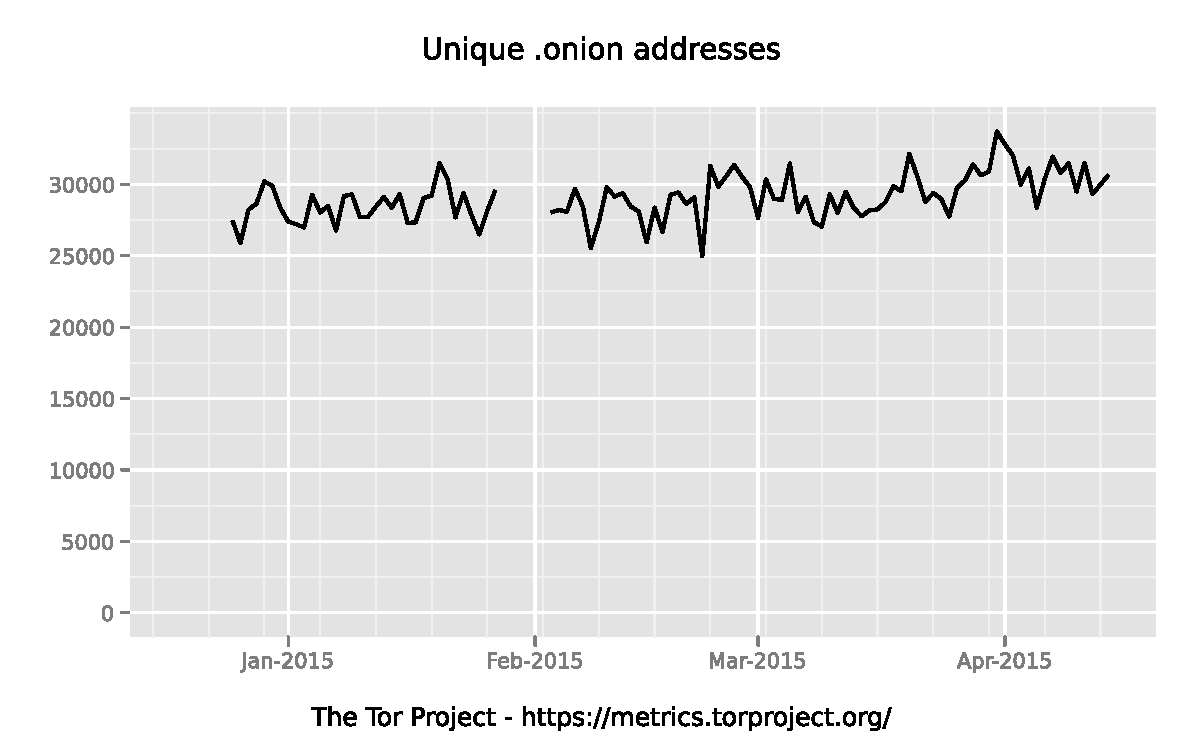
\includegraphics[width=0.45\textwidth]{../images/Tor/onion_2014-10_2015-04.pdf}
	\caption{The number of unique .onion addresses seen in Tor's distributed hashtable between January through April 2015.\cite{TorMetrics}\cite{kadianakis2015extrapolating}}
\end{figure}

\section{Design Objectives} % done

Tor's privacy-enhanced environment introduces a distinct set of challenges that must be met by any additional functionality. Here we enumerate a list of requirements that must be met by any DNS applicable to Tor hidden services. In Section \ref{sec:ExistingWorks} we analyse several existing prominent naming systems and show how these systems do not meet these requirements, and in Section \ref{sec:Solution} and \ref{sec:Analysis} we demonstrate how we overcome them with OnioNS.

\begin{enumerate}[noitemsep]
	\item \textbf{The system must support anonymous registrations.} The system should not require any personally-identifiable or location information from the registrant. Tor hidden services publicize no more information than a public key and Introduction Points.
	\item \textbf{The system must support privacy-enhanced queries.} Clients should be anonymous, indistinguishable, and unable to be tracked by name servers.
	\item \textbf{Clients must be able to authenticate registrations.} Clients must be able to verify that the domain-destination pairing that they receive from name servers is authentic relative to the authenticity of the destination server.
	\item \textbf{Domain names must be globally unique.} Any domain name of global scope must point to at most one server. In the case of naming systems that generate names via cryptographic hashes, the domain name key-space must be of sufficient length to be remain resistant to at least collision and second pre-image attacks.
	\item \textbf{The system must be distributed.} Systems with root authorities have distinct disadvantages compared to distributed networks: specifically, central authorities have absolute control over the system and root security breaches could easily compromise the integrity of the entire system. Root authorities may also be able to compromise user privacy or may not allow anonymous registrations. For these reasons, naming systems with central authorities can safely be considered ill-suited for hidden services.
	\item \textbf{The system must be relatively easy to use.} It should be assumed that users are not security experts or have technical backgrounds. The system must resolve protocols with minimal input from the user and hide non-essential details.
	\item \textbf{The system must be backwards compatible.} Naming systems for Tor must preserve the original Tor hidden service protocol, making the DNS optional but not required.
	\item \textbf{The system must not introduce significant burdens to clients.} In most realistic environments clients have neither the bandwidth nor storage capacity to hold the system's entire database, nor the capability of meeting significant computation or memory demands.
\end{enumerate}

\section{Existing Works} % done
\label{sec:ExistingWorks}

Vanity key generators (e.g. Shallot\cite{KatmagicShallot}) attempt to find by brute-force an RSA key that generates a partially-desirable hash. Vanity key generators are commonly used by hidden service operators to improve the recognition of their hidden service, particularly for higher-profile services.\cite{syversongenuine} For example, a hidden service operator may wish to start his service's address with a meaningful noun so that others may more easily recognize it. However, these generators are only partially successful at enhancing readability because the size of the domain key-space is too large to be fully brute-forced in any reasonable length of time. If the address key-space was reduced to allow a full brute-force, the system would fail to be guaranteed collision-free. Nicolussi suggested changing the address encoding to a delimited series of words, using a dictionary known in advance by all parties.\cite{nicolussi2011human} Like vanity key generators, Nicolussi's encoding partially improves the recognition and readability of an address but does nothing to alleviate the logistic problems of manually entering in the address into the Tor Browser. The key-space is not changed and is again too large for hidden service operators to select many meaningful words, making these attempts purely cosmetic and not a full solution.

The Internet DNS is another one candidate and is already well established as a fundamental abstraction layer for Internet routing. However, despite its widespread use and extreme popularity, the Internet DNS suffers from several significant shortcomings and fundamental security issues that make it inappropriate for use by Tor hidden services. With the exception of extensions such as DNSSEC, the Internet DNS by default does not use any cryptographic primitives. DNSSEC is primarily designed to prevent forgeries and DNS cache poisoning from intermediary name servers and it does not provide any degree of query privacy.\cite{wachs2014censorship} Additional extensions and protocols such as DNSCurve\cite{bernstein2009dnscurve} have been proposed, but DNSSEC and DNSCurve are optional and have not yet seen widespread full deployment across the Internet. The lack of default security in Internet DNS and the financial expenses involved with registering a new TLD casts significant doubt on the feasibility of using it for Tor hidden services. Cachin and Samar\cite{cachin2004secure} extended the Internet DNS and decreased the attack potential for authoritative name servers via threshold cryptography, but the lack of privacy in the Internet DNS and the logistical difficulty in globally implementing their work prevents us from using their system for hidden services.

The GNU Name System\cite{wachs2014censorship} (GNS) is another zone-based alternative DNS. GNS describes a hierarchical zones of names with each user managing their own zone and distributing zone access peer-to-peer within social circles. While GNS' design guarantees the uniqueness of names within each zone and users are capable of selecting meaningful nicknames for themselves, GNU does not guarantee that names are \emph{globally} unique. Furthermore, the selection of a trustworthy zone to use would be a significant challenge for using GNS for Tor hidden services and such a selection no longer makes the system distributed. Awerbuch and Scheideler,\cite{awerbuch2004group} constructed a distributed peer-to-peer naming system, but like GNS, made no guarantee that domain names would be globally unique.

Namecoin\cite{NamecoinHome}\cite{jacobs2014providing} was an early fork of Bitcoin\cite{nakamoto2008bitcoin} and is noteworthy for achieving all three properties of Zooko's Triangle. Namecoin holds information transactions in a distributed ledger known as a blockchain. Storing textual information such as a domain registration consumes some Namecoins, a unit of currency. While Namecoin is often advertised as capable of assigning names to Tor hidden services, it has several practical issues that make it generally infeasible to be used for that purpose. First, to authenticate registrations, clients must be able to prove the relationship between a Namecoin owner's secp256k1 ECDSA key and the target hidden service's RSA key: constructing this relationship is non-trivial. Second, Namecoin generally requires users to pre-fetch the blockchain which introduces significant logistical issues due to high bandwidth, storage, and CPU load. Third, although Namecoin supports anonymous ownership of information, it is non-trivial to anonymously purchase Namecoins, thus preventing domain registration from being truly anonymous. These issues prevent Namecoin from being a practical alternative DNS for Tor hidden service. However, our work shares some design principles with Namecoin.

\section{Challenges}

\subsection{Zooko's Triangle} % done

In 2001, Zooko Wilcox-O'Hearn described three desirable properties for any persistent naming system: distributed design, assignment of human-meaningful names, and globally unique names. In a statement now known as Zooko's Triangle,\cite{ferdous2009security}\cite{stiegler2005petname} he claimed any naming system could only achieve two of these properties. This is illustrated in Figure \ref{fig:ZookosTriangle}.

\begin{figure}[htbp]
	\centering
	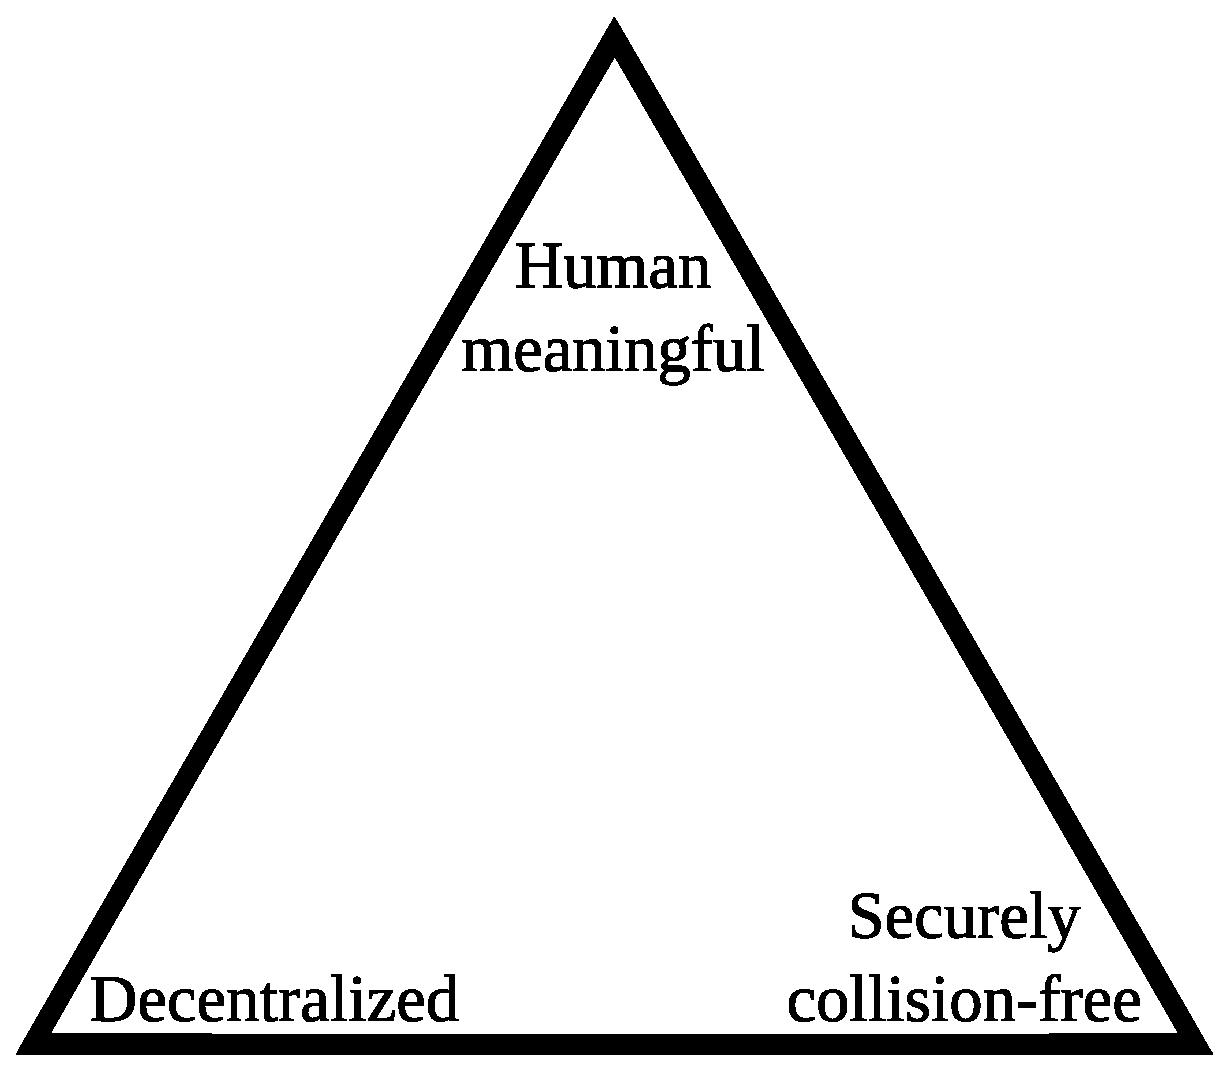
\includegraphics[width=0.3\textwidth]{../images/Zooko.eps}
	\caption{Zooko's Triangle.}
	\label{fig:ZookosTriangle}
\end{figure}

Some examples of naming systems that achieve only two of these properties include:

\begin{itemize}[noitemsep]
	\item \textbf{Securely unique and human-meaningful} \\ --- Internet domain names and GNS.
	\item \textbf{Decentralized and human-meaningful} \\ --- Human names and nicknames.
	\item \textbf{Securely unique and decentralized} \\ --- Tor hidden service .onion addresses.
\end{itemize}

Petnames, such as Namecoin and OnioNS, are systems that achieve all three properties of Zooko's Triangle.

\subsection{Authenticated Denial-of-Existence} % done

If a naming system provides authentication, clients should be able to verify the authenticity of existing domain names and authenticate a denial-of-existence claim by their name server. On the Internet, the former is addressed by SSL certificates and a chain of trust to root Certificate Authorities, while the latter remains a possible attack vector. DNSSEC includes an extension for Hashed Authenticated Denial of Existence (NSEC3) which provides signed non-existence claims on a per-domain basis. However, DNSSEC has not seen widespread use, storing per-domain denial-of-existence records introduces significant storage requirements, and to our knowledge no alternative DNS provides mechanisms for authenticated denial-of-existence. Closing this attack vector is not easy; the na\"{i}ve solution of generating proof individually or en-masse for every non-existent domain is infeasible since the number of possible domain names is likely too large to practically enumerate.

\newpage

\section{Assumptions and Threat Model} % done

\begin{enumerate}[noitemsep,nolistsep]
	\item We assume that Tor provides privacy and anonymity; if Alice constructs a three-hop Tor circuit to Bob with modern Tor cryptographic protocols and sends a message $ m $ to Bob, we assume that Bob can learn no more about Alice than the contents of $ m $. This implies that if $ m $ does not contain identifiable information, Alice is anonymous from Bob's perspective, regardless of if $ m $ is exposed to an attacker, Eve. Identifiable information in $ m $ is outside of Tor's scope, but we do not introduce any protocols that cause this scenario.
	\item We assume reliable cryptography; namely that Eve cannot break standard cryptographic primitives such as AES, SHA-2, RSA, Curve25519, Ed25519, the scrypt key derivation function, or Tor protocols derived from these primitives. We assume that Eve maintains no backdoors or knows secret software breaks in the Botan or the OpenSSL implementations of these primitives.
	\item We assume that not all Tor routers are honest; that Eve controls some percentage of Tor routers such that Eve's routers may actively collude. Routers may also be semi-honest; wiretapped but not capable of violating protocols. However, the percentage of dishonest and semi-honest routers is small enough to avoid violating our first assumption.
	\item We assume a fixed percentage of dishonest and semi-honest routers; namely that the percentage of routers under an Eve's control does not increase in response to the inclusion of OnionNS into Tor infrastructure. This assumption simplifies our threat model analysis but we consider it realistic because while Tor traffic is purposely secret as it travels through the network, we consider OnioNS information public so we don't consider the inclusion of OnioNS a motivating factor to Eve.
	\item If $ C $ is a Tor network status consensus, $ Q $ is an $ M $-sized set randomly but deterministically selected from the Fast and Stable routers listed in $ C $, and $ Q $ is under the influence of one or more adversaries, we assume that the largest subset of agreeing routers in $ Q $ are at least semi-honest.
\end{enumerate}

\section{Solution}
\label{sec:Solution}

\subsection{Overview} % done

\begin{figure}[htbp]
	\centering
	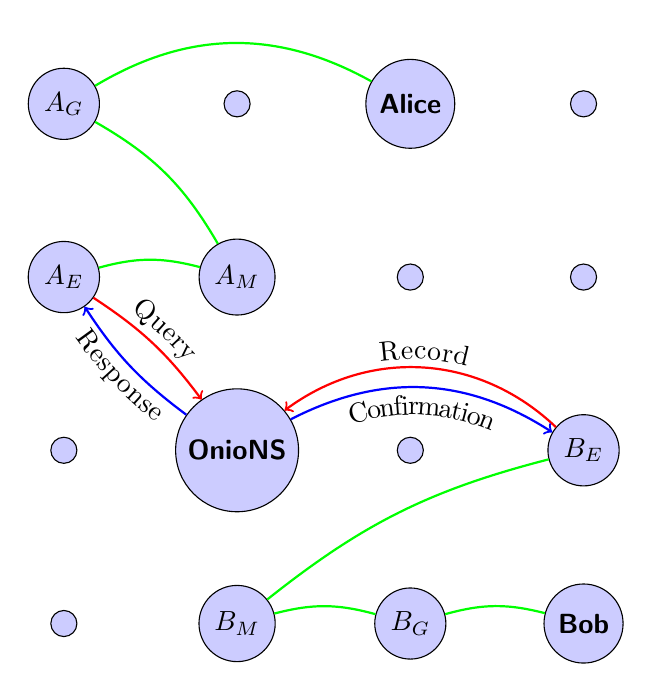
\begin{tikzpicture}[->, node distance=2.2cm, main node/.style={circle, fill=blue!20, draw, font=\sffamily\bfseries}]

			\node[main node] (1) {$ A_{G} $};
			\node[main node] (2) [right of=1] {};
			\node[main node] (3) [right of=2] {Alice};
			\node[main node] (4) [right of=3] {};

			\node[main node] (5) [below of=1] {$ A_{E} $};
			\node[main node] (6) [right of=5] {$ A_{M} $};
			\node[main node] (7) [right of=6] {};
			\node[main node] (8) [right of=7] {};

			\node[main node] (9) [below of=5] {};
			\node[main node] (10) [right of=9] {OnioNS};
			\node[main node] (11) [right of=10] {};
			\node[main node] (12) [right of=11] {$ B_{E} $};

			\node[main node] (13) [below of=9] {};
			\node[main node] (14) [right of=13] {$ B_{M} $};
			\node[main node] (15) [right of=14] {$ B_{G} $};
			\node[main node] (16) [right of=15] {Bob};

			% Alice-OnioNS conversation
			\tikzstyle{EdgeStyle}=[bend right, -, green]
			\Edge[](3)(1)
			\tikzstyle{EdgeStyle}=[bend left=15, -, green]
			\Edge[](1)(6)
			\Edge[](5)(6)
			\draw[thick, ->, red, postaction={decorate, decoration={text along path, text align=center, text={Query}, raise=4pt}}] (5) to [bend left=10] (10){};
			\draw[thick, <-, blue, postaction={decorate, decoration={text along path, text align=center, text={Response}, raise=-9pt}}] (5) to [bend right=10] (10){};

			% Bob-OnioNS conversation
			\tikzstyle{EdgeStyle}=[bend right=15, -, green]
			\Edge[](16)(15)
			\Edge[](15)(14)
			\tikzstyle{EdgeStyle}=[bend left=12, -, green]
			\Edge[](14)(12)
			\draw[thick, red, <-, postaction={decorate, decoration={text along path, text align=center, text={Record}, raise=3pt}}] (10) to [bend left=40] (12){};
			\draw[thick, blue, ->, postaction={decorate, decoration={text along path, text align=center, text={Confirmation}, raise=-10pt}}] (10) to [bend left=30] (12){};

		\end{tikzpicture}
	\caption{Bob uses a Tor circuit ($ B_{G} $, $ B_{M} $, $ B_{E} $) to anonymously broadcast a record to OnioNS. Alice uses her own Tor circuit ($ A_{G} $, $ A_{M} $, $ A_{E} $) to query the system for a domain name, and she is given Bob's record in response. Then Alice connects to Bob by Tor's hidden service protocol.}
	\label{fig:basicDesign}
\end{figure}

We propose the Onion Name System (OnioNS) as an abstraction layer to hidden service addresses and introduce ``.tor'' as a new pseudo-TLD for this purpose. First, Bob generates and self-signs a \emph{Record}, containing an association between a meaningful second-level domain name and his .onion address. Without loss of generality, let this be ``example.tor $ \rightarrow $ example0uyw6wgve.onion''. We introduce a proof-of-work scheme that requires Bob to expend computational and memory resources to claim ``example.tor'', a more privacy-enhanced alternative to financial compensation to a central authority. Proof-of-work systems are noteworthy for their asymmetry: they require the issuer to spend effort to find an answer to a moderately hard computational problem, but once solved can be easily verified correct by any recipient. The requirement of proof-of-work fulfils three main purposes:

\begin{enumerate}[noitemsep,nolistsep]
	\item Significantly reduces the threat of denial-of-service flood attack.
	\item Introduces a barrier-of-entry that encourages the utilization of domain names and the availability of the underlying hidden services.
	\item Increases the difficulty of domain squatting.
\end{enumerate}

Second, Bob uses a Tor circuit to anonymously transmit his Record to an authoritative short-lived subset of OnioNS servers, known as the \emph{Quorum}, inside the Tor network. The Quorum archive Bob's Record in a sequential public ledger known as a \emph{Pagechain}, of which each OnioNS node holds their own local copy. Bob's Record is received by all Quorum nodes and share signatures of their knowledge with each other, so they maintain a common database. Quorum nodes are not name servers, so let Charlie be a name server outside the Quorum and assume that Charlie stays synchronized with the Quorum.

Third, Alice, uses a Tor client to anonymously connect to Charlie, then asks Charlie for ``example.tor''. Alice receives Bob's Record, verifies it signature and proof-of-work, and follows the association to ``example0uyw6wgve.onion''. As Bob's Record is self-signed using Bob's private key, Alice can verify the Record's authenticity. Finally, Alice uses this address and the Tor hidden service protocol to contact Bob. Note that Alice does not have to resort to using ``example0uyw6wgve.onion'', rather that Bob can be successfully referenced by ``example.tor''. We illustrate the OnioNS overview in Figure \ref{fig:basicDesign}.

\subsection{Cryptographic Primitives} % done

OnionNS makes use of cryptographic hash algorithms, digital signatures, proof-of-work, and a pseudorandom number generator. We require that Tor routers generate an Ed25519\cite{bernstein2011high} keypair and distribute the public key via the consensus document. We note that because the Ed25519 elliptic curve is birationally equivalent to Curve25519 and because it is possible to convert Curve25519 to Ed25519 in constant time, we can theoretically use existing NTor keys for digital signatures. However, we refrain from this because to our knowledge there is no formal analysis that demonstrates that this a cryptographically secure operation. Therefore we require Tor to introduce Ed25519 keys to all Tor routers. If this is infeasible, Ed25519 can be substituted with RSA in all instances.

\begin{itemize}[noitemsep,nolistsep]
	\item Let $ H(x) $ be a cryptographic hash function. In our reference implementation we define $ H(x) $ as SHA-384.
	\item Let $ S_{\mathit{RSA}}(m, r) $ be a deterministic RSA digital signature function that accepts a message $ m $ and a private RSA key $ r $ and returns an RSA digital signature. Let $ S_{d}(m, r) $ use $ H(x) $ as a digest function on $ m $ in all use cases. In our reference implementation we define $ S_{d}(m, r) $ as EMSA-PSS, (EMSA4) a probabilistic signature scheme defined by PKCS1 v2.1 and republished in 2003's RFC 3447.
	\item Let $ V_{\mathit{RSA}}(m, E) $ validate an RSA digital signature by accepting a message $ m $ and a public key $ R $, and return true if and only if the signature is valid.
	\item Let $ S_{\mathit{ed}}(m, e) $ be an Ed25519 digital signature function that accepts a message $ m $ and a private key $ e $ and returns a 64-byte digital signature. Let $ S_{\mathit{ed}}(m, e) $ use $ H(x) $ as a digest function on $ m $ in all use cases.
	\item Let $ V_{\mathit{ed}}(m, E) $ validate an Ed25519 digital signature by accepting a message $ m $ and a public key $ E $, and return true if and only if the signature is valid.
	\item Let $ \mathrm{PoW}(k) $ be a one-way collision-free function that accepts an input key $ k $ and returns a deterministic output. Our reference implementation uses the scrypt key derivation function with a fixed salt.
	\item Let $ \mathit{R}(s) $ be a pseudorandom number generator that accepts an initial seed $ s $ and returns a list of numerical pseudorandom numbers. $ \mathit{R}(s) $ does not need to be cryptographically secure. We suggest MT19937, commonly known as the Mersenne Twister. This generator is widely used throughout most programming languages and is well known for its speed, long period, and the high quality of its pseudorandom output.\cite{matsumoto1998mersenne}
\end{itemize}

 \subsection{Definitions} % done

\begin{description}
	\item[domain name] \hfill \\
		The syntax of OnioNS domain names mirrors the Internet DNS; we use a sequence of name-delimiter pairs with a .tor pseudo-TLD. The Internet DNS defines a hierarchy of administrative realms that are closely tied to the depth of each name. By contrast, OnioNS makes no such distinction; we let hidden service operators claim second-level names and then control all names of greater depth under that second-level name.

	\item[Record] \hfill \\
		A \emph{Record} contains \emph{nameList}, a one-to-one map of .tor pseudo-TLD domain names and .tor or .onion pseudo-TLD destinations; \emph{contact}, Bob's PGP key fingerprint if he chooses to disclose it; \emph{consensusHash}, the hash of the consensus document that generated the current Quorum; \emph{nonce}, four bytes used as a source of randomness for the proof-of-work; \emph{pow}, the output of $ \mathrm{PoW}(i) $; \emph{recordSig}, the output of $ S_{d}(m, r) $ where $ m = \mathit{nameList} \concat \mathit{timestamp} \concat \mathit{consensusHash} \concat \mathit{nonce} \concat \mathit{pow} $ and $ r $ is the hidden service's private RSA key; and \emph{pubHSKey}, Bob's public hidden service RSA key.

	\item[Snapshot] \hfill \\
		A \emph{Snapshot} contains \emph{originTime}, the Unix time when the snapshot was first created; \emph{recentRecords}, an array list of Records in reverse chronological order; \emph{fingerprint}, the Tor fingerprint of the router maintaining this Snapshot; and  \emph{snapshotSig}, the output of $ S_{\mathit{ed}}(\mathit{originTime} \concat \mathit{recentRecords} \concat \mathit{fingerprint}], e) $ where $ e $ is the router's private Ed25519 key.

	\item[Page] \hfill \\
		A \emph{Page} contains \emph{prevHash}, the output of $ H(\emph{prevHash} \concat \emph{recordList} \concat \emph{consensusHash}) $ of a previous Page; \emph{recordList}, a deterministically-sorted array list of Records; \emph{consensusHash}, the hash of the consensus document that generated the current Quorum; \emph{fingerprint}, the Tor fingerprint of the router maintaining this Page; and \emph{pageSig}, the output of $ S_{\mathit{ed}}(H(\mathit{prevHash} \concat \mathit{recordList} \concat \mathit{consensusHash})], e) $ where $ e $ is the router's private Ed25519 key.
		
		\emph{prevHash} links Pages over time, forming an append-only public ledger known as an \emph{Pagechain}. In contrast to existing cryptocurrencies such as Namecoin, we bound the Pagechain to a finite length, forcing hidden service operators to renew their domain periodically to avoid it being dropped from the network. In correspondence with our last security assumption, \emph{prevHash} must reference a Page that is both valid and maintained by the largest number of Quorum members, as illustrated in Figure \ref{fig:sideChains}. As \emph{prevHash} does not include the router-specific \emph{fingerprint} and \emph{pageSig} fields, \emph{prevHash} is equal across all Quorum members maintaining that Page.

	\item[Mirror] \hfill \\
		A \emph{Mirror} is any name server that holds a complete copy of the Pagechain and maintains synchronization against the Quorum. The primary job of a Mirror is to respond to queries. We note that Mirrors may be outside the Tor network, but in this work we do not specify any protocols for this scenario.

	\item[Quorum Candidate] \hfill \\
		A \emph{Quorum Candidates} are \emph{Mirrors} that provide proof in the network status consensus that they are an up-to-date Mirror in the Tor network and that they have sufficient CPU and bandwidth capabilities to handle OnioNS communication in addition to their regular Tor duties.

	\item[Quorum] \hfill \\
		A \emph{Quorum} is a subset of Quorum Candidates who have active responsibility over maintaining the master Pagechain. Each Quorum node actively its own Page, which has a lifetime of that Quorum. The Quorum is randomly chosen from Quorum Candidates.
\end{description}

All textual databases are encoded in JSON. JSON is significantly more compact than XML, but retains readability. Its support of basic primitive types is highly applicable to our needs. Additionally, we consider the JSON format safer than byte-level encoding.

%\begin{figure}[htdp]
%	\begin{minipage}[b]{0.5\textwidth}
%		\centering
%		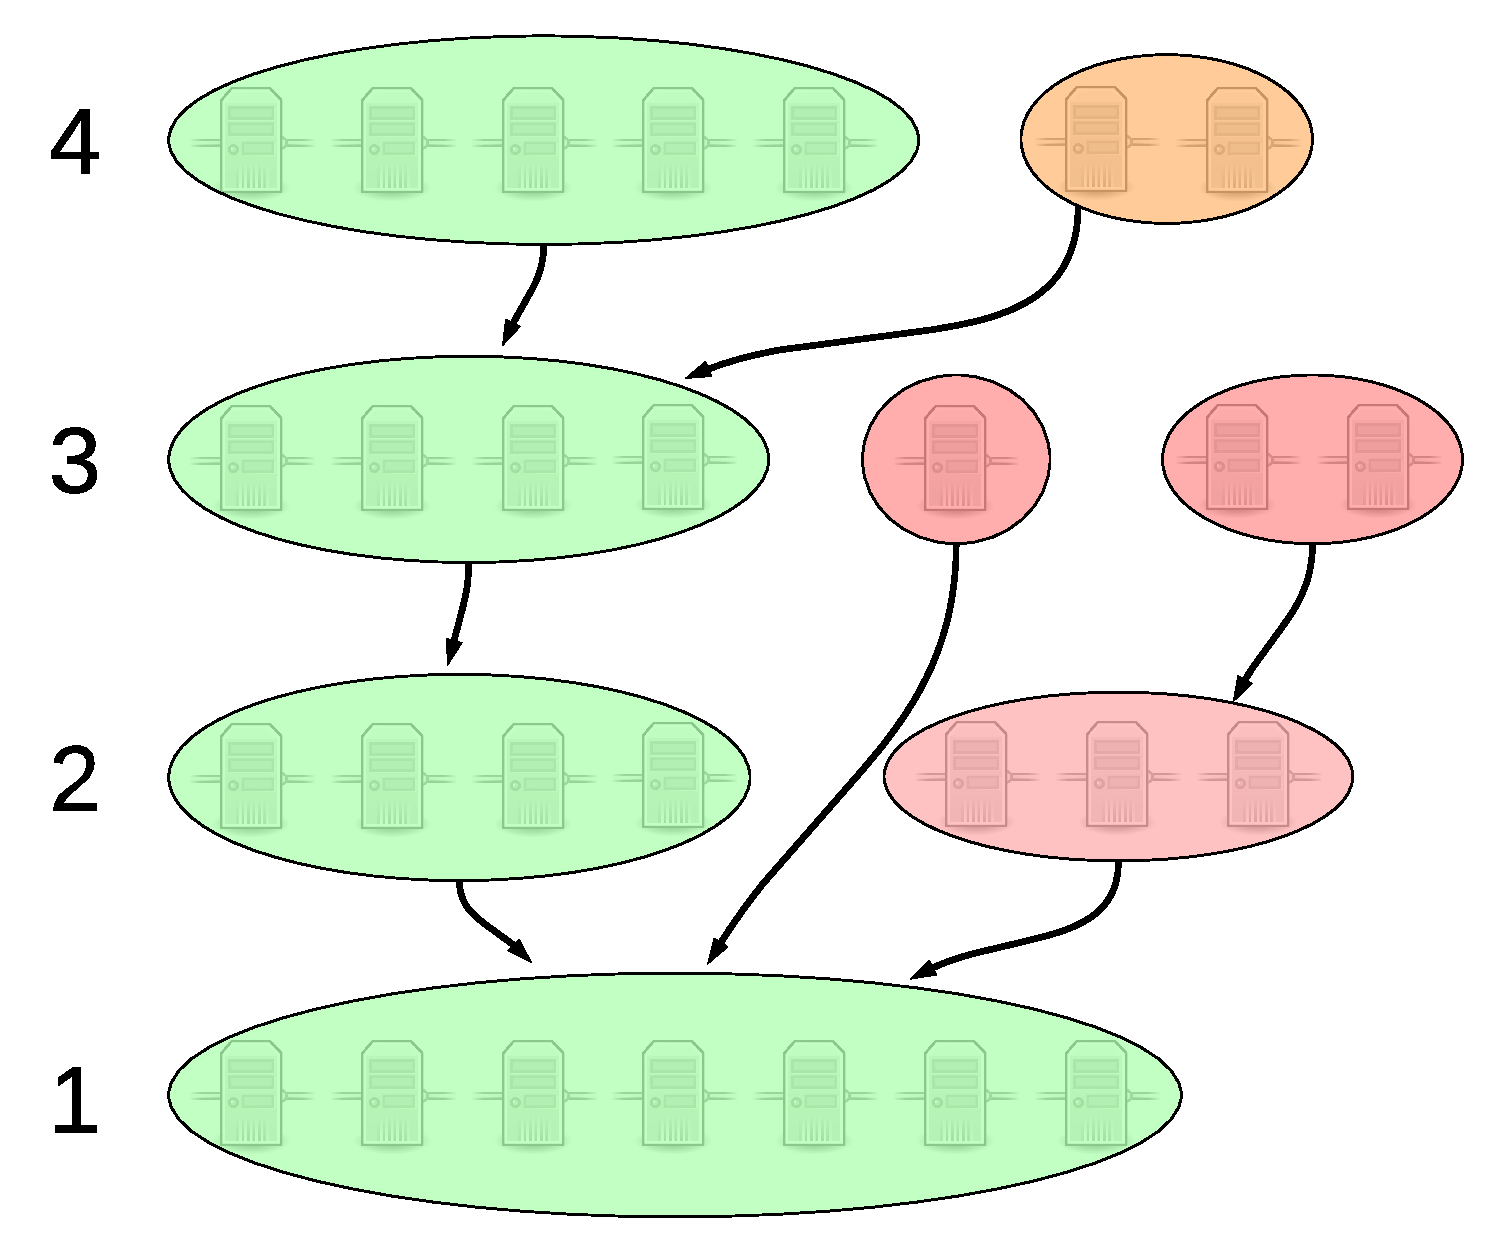
\includegraphics[width=0.7\textwidth]{../images/LucidCharts/Page-chain2.pdf}
%		\caption{An example Pagechain across four Quorums with three side-chains. The valid master Pagechain from honest Quorum nodes (green) resists corruption from maliciously-colluding nodes (red) and malfunctioning nodes (orange).}
%	\end{minipage}
%	\vspace{0.5cm}
%	\begin{minipage}[b]{0.5\textwidth}
%		\centering
%		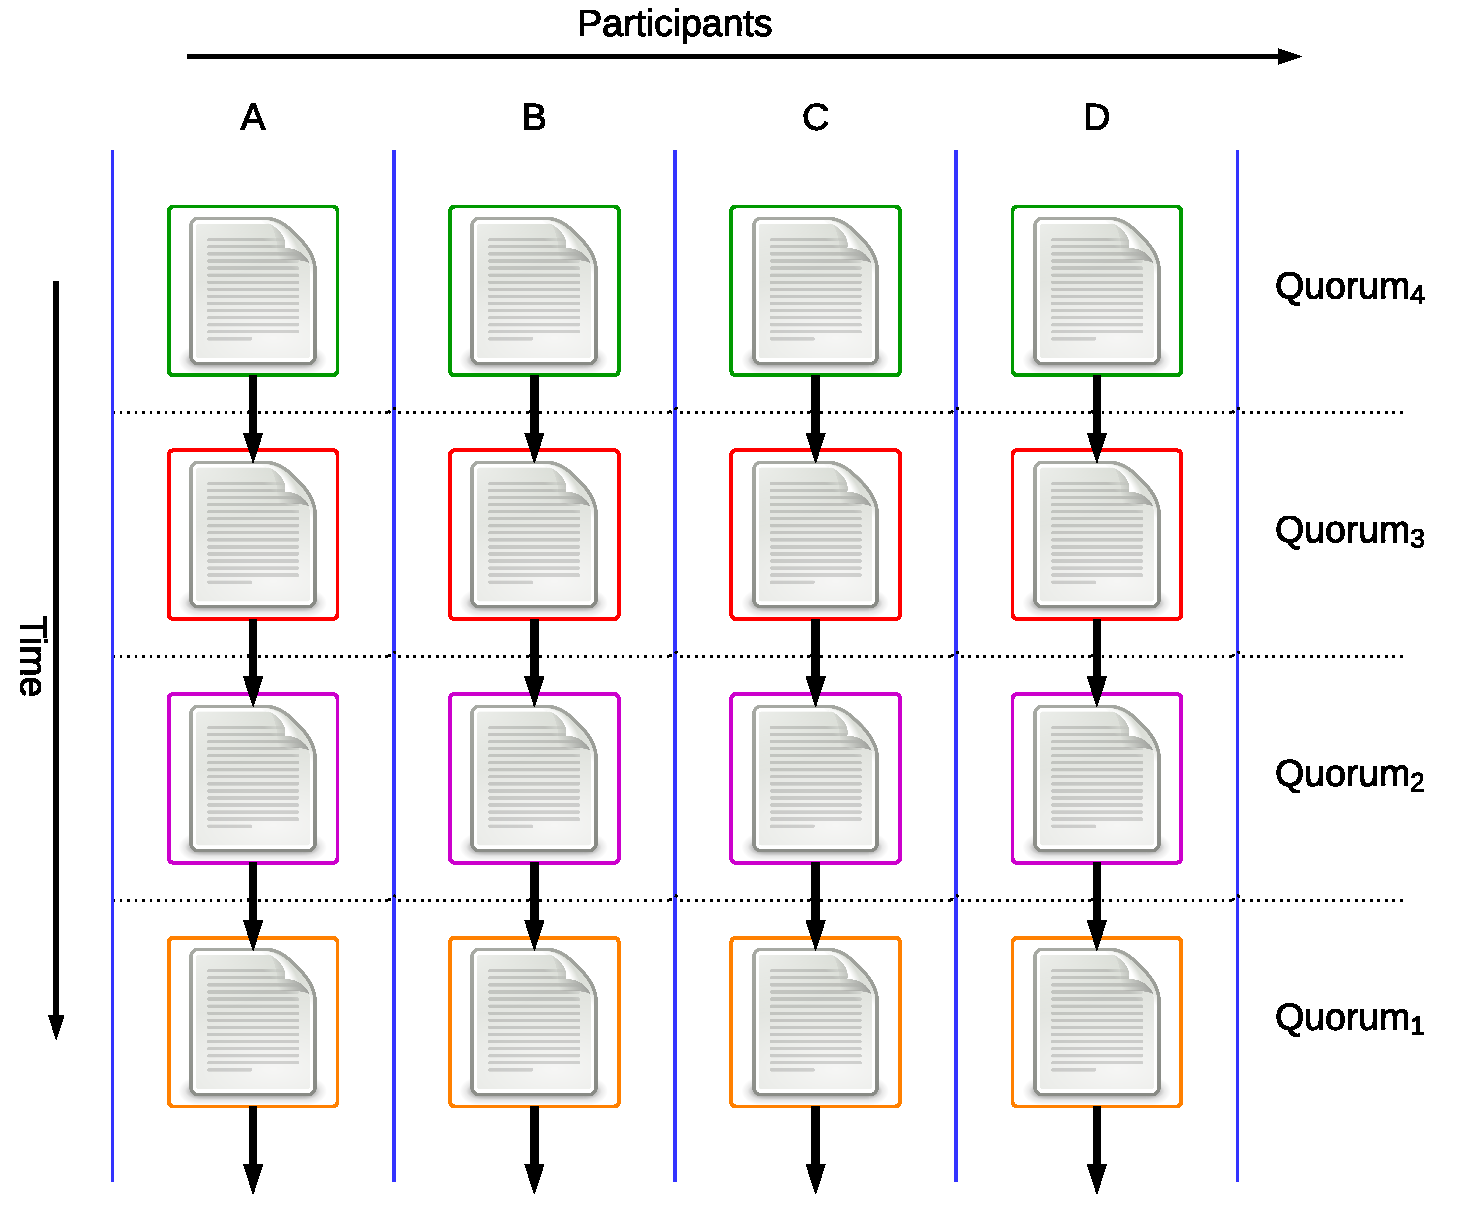
\includegraphics[width=0.9\textwidth]{../images/LucidCharts/Data-Structure-Overview.pdf}
%	\caption{The master Pagechain is one-dimensional but spans across the network as each Mirror holds a copy. Each Page is maintained by a respective Quorum.}
%	\end{minipage}
%\end{figure}

\begin{figure}[h]
	\centering
	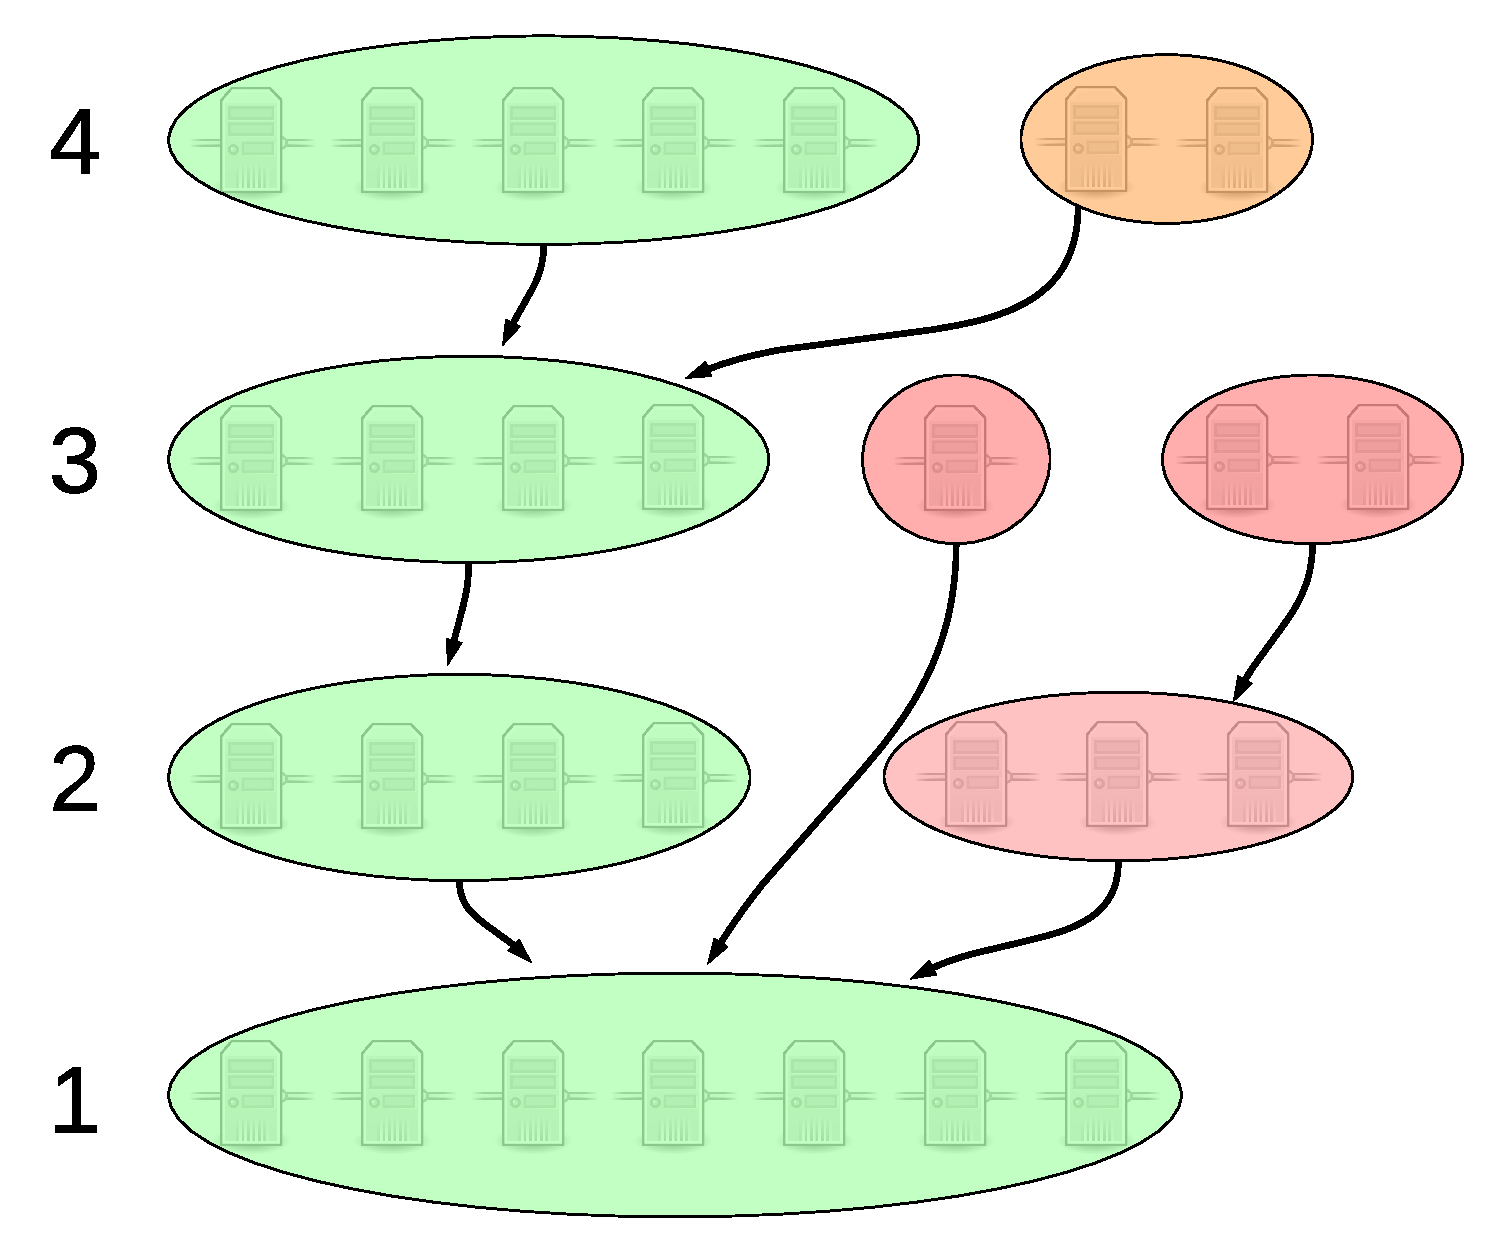
\includegraphics[width=0.85\linewidth]{../images/LucidCharts/Page-chain2.pdf}
	\caption{An example Pagechain across four Quorums with three side-chains. The valid master Pagechain from honest Quorum nodes (green) resists corruption from maliciously-colluding nodes (red) and malfunctioning nodes (orange).}
	\label{fig:sideChains}
\end{figure}

\begin{figure}[h!]
	\centering
	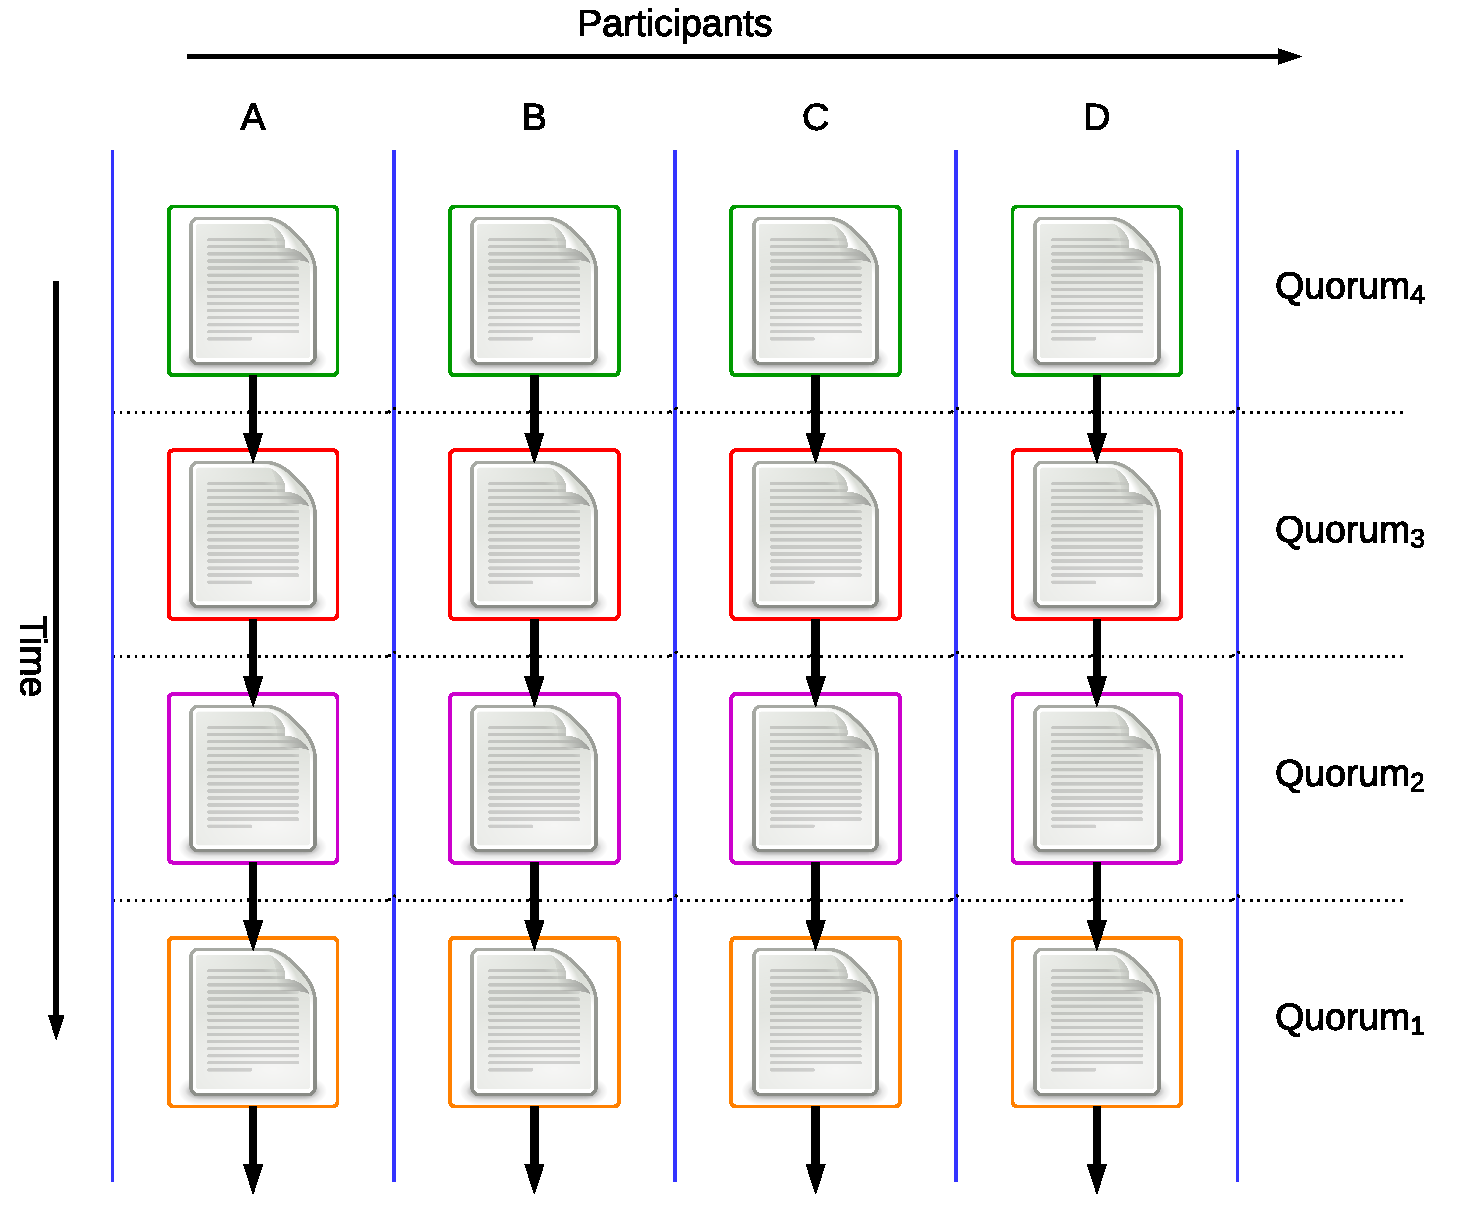
\includegraphics[width=1\linewidth]{../images/LucidCharts/Data-Structure-Overview.pdf}
	\caption{The master Pagechain is one-dimensional but spans across the network as each Mirror holds a copy. Each Page is maintained by a respective Quorum.}
\end{figure}

\subsection{Symbols} % done

\begin{itemize}[noitemsep,nolistsep]
	\item Let $ L_{Q} $ represent size of the Quorum.
	\item Let $ L_{T} $ represent the number of routers in the Tor network.
	\item Let $ L_{P} $ represent the maximum number of Pages in the Pagechain.
	\item Let $ q $ be an Quorum iteration counter.
	\item Let $ \Delta q $ be the lifetime of a Quorum in days: every $ \Delta q $ days $ q $ is incremented by one and a new Quorum is chosen.
	\item Let $ s $ be a Snapshot iteration counter.
	\item Let $ \Delta s $ be the lifetime of a Snapshot in minutes.
\end{itemize}

\newpage

\subsection{Protocols} % done

We now describe the protocols fundamental to OnioNS functionality. Further readings on our protocols may be found at the OnioNS hidden service, \url{http://onions55e7yam27n.onion}.

\subsubsection{Record Generation} % done

Bob must first generate a valid Record to claim a second-level domain name for his hidden service. The validity of his Record is checked by both Mirrors and clients, so Bob must follow this protocol.

\begin{enumerate}[noitemsep]
	\item Bob constructs the \emph{nameList} domain-destination associations. He must include at least one second-level domain name. Each domain name can be up to 128 characters and contain any number of names.
	\item Bob optionally provides his PGP key fingerprint in \emph{contact}.
	\item Bob sets \emph{consensusHash} to the output of $ H(x) $, where $ x $ is the consensus documents published at 00:00 GMT on day $ \floor[\big]{\frac{q}{\Delta q}} $.
	\item Bob initially defines \emph{nonce} as four zeros.
	\item Let $ \mathit{central} $ be $\mathit{type} \concat \mathit{nameList} \concat \mathit{contact} \concat \mathit{timestamp} \concat \mathit{consensusHash} \concat \mathit{nonce} $.
	\item Bob sets \emph{pow} as $ \mathrm{PoW}(\mathit{central}) $.
	\item Bob sets \emph{recordSig} as the output of $ S_{d}(m, r) $ where $ m = \mathit{central} \concat \mathit{pow} $ and $ r $ is Bob's private RSA key.
	\item Bob saves the PKCS.1 DER encoding of his RSA public key in \emph{pubHSKey}.
\end{enumerate}

The Record is valid when $ H(\mathit{central} \concat \mathit{pow} \concat \mathit{recordSig}) \leq 2^{\mathit{d} * \mathit{c}} $ where \emph{d} is a fixed constant that specifies the work difficulty and \emph{c} is the number of second-level domain names claimed in the Record. This also requires Bob to increment \emph{nonce} and resign his Record at every iteration of $ \mathrm{PoW}(\mathit{central}) $.

%\subsubsection{Record Broadcast}
%
%\begin{enumerate}[noitemsep,nolistsep]
%	\item Bob derives the current Quorum by the Quorum Derivation protocol described in section \ref{sec:ProtoTorClients}.
%	\item Bob constructs a circuit, $ c_{1} $, to a Mirror node $ m_{1} $.
%	\item Bob asks for and receives from $ c_{1} $ the $ h_{j} = H(\mathit{prevHash} \concat \mathit{recordList} \concat \mathit{consensusHash}) $ hash and \emph{pageSig} (the Ed25519 signature on that hash) from each Quorum node.
%	\item Bob confirms that $ V_{\mathit{ed}}(h_{j}, E) $ returns true for each $ h_{j} $ and defines $ U $ as the largest set of Quorum nodes that have the same hash.
%	\item Bob randomly chooses a node $ n_{1} $ from $ U $ and builds a circuit to it, $ c_{2} $.
%	\item Bob uploads his Record through $ c_{2} $ to $ n_{1} $.
%	\item Bob waits up to $ \Delta s $ minutes for the next $ s $ flood iteration.
%	\item Bob uses $ c_{1} $ to ask $ m_{1} $ for any second-level domain name contained in his Record.
%	\item Bob has confirmation that his Record was accepted and processed by the Quorum if $ m_{1} $ returns the Record he uploaded.
%	\item If $ m_{1} $ does not return Bob's Record, he can either query another Mirror or repeat this procedure and broadcast to a different Quorum node.
%\end{enumerate}

%\begin{figure}[htbp]
%	\centering
%	\begin{tikzpicture}[->, node distance=2.2cm, main node/.style={circle, fill=blue!20, draw, font=\sffamily\bfseries}]
%
%			\node[main node] (1) {$ Q_{1} $};
%			\node[main node] (2) [right of=1] {$ Q_{2} $};
%			\node[main node] (3) [right of=2] {};
%			\node[main node] (4) [right of=3] {$ Q_{3} $};
%
%			\node[main node] (5) [below of=1] {};
%			\node[main node] (6) [right of=5] {$ Q_{4} $};
%			\node[main node] (7) [right of=6] {};
%			\node[main node] (8) [right of=7] {};
%
%			\node[main node] (9) [below of=5] {$ R_{M} $};
%			\node[main node] (10) [right of=9] {};
%			\node[main node] (11) [right of=10] {$ R_{E} $};
%			\node[main node] (12) [right of=11] {$ Q_{5} $};
%
%			\node[main node] (13) [below of=9] {};
%			\node[main node] (14) [right of=13] {};
%			\node[main node] (15) [right of=14] {$ R_{E} $};
%			\node[main node] (16) [right of=15] {HS};
%
%			% draw 1st and 2nd part of circuit
%			\tikzstyle{EdgeStyle}=[bend right=12, -, green]
%			\Edge[](16)(15)
%			\Edge[](9)(15)
%
%			% draw last part of circuit
%			\tikzstyle{EdgeStyle}=[bend left=17, -, green]
%			\Edge[](9)(11)
%
%			% draw record moving from exit to 1st q. node
%			\draw[thick, red, <-, postaction={decorate, decoration={text along path, text align=center, text={Record}, raise=3pt}}] (6) to [bend right=15] (11){};
%
%			% draw verification with second q. node
%			\draw[thick, red, ->, postaction={decorate}] (12) to [bend left=15] (11){};
%
%			% draw upper left propegation
%			\tikzstyle{EdgeStyle}=[bend left=12, ->, blue]
%			\Edge[](6)(2)
%			\Edge[](6)(1)
%
%			% draw upper right propegation
%			\tikzstyle{EdgeStyle}=[bend left=20, ->, blue]
%			\Edge[](6)(12)
%			\draw[thick, blue, postaction={decorate, decoration={text along path, text align=center, text={Snapshot}, raise=3pt}}] (6) to [bend right=18] (4){};
%
%		\end{tikzpicture}
%	\caption{Bob uses his existing circuit (green) to inform Quorum node $ Q_{4} $ of the new record. $ Q_{4} $ then floods it via Snapshots to all other Quorum nodes. Each node stores it in their own Page for long-term storage. Bob confirms from another Quorum node $ Q_{5} $ that his Record has been received.}
%	\label{fig:recordBroadcast}
%\end{figure}

\subsubsection{Page Selection} % done

New Quorum nodes must select a Page from the previous Quorum to reference when generating a fresh Page. To reduce the chances of compromise, we select from the previous Quorum a Page that is both valid and maintained by the largest number of Quorum members. Mirrors must then verify this selection retrospectively for each Page chronologically in the Pagechain.

\begin{enumerate}[noitemsep,nolistsep]
	\item Charlie obtains the set of Pages maintained by $ \mathit{Quorum}_{q} $.
	\item Charlie obtains the consensus $ \mathit{cd} $ issued on day $ \floor[\big]{\frac{q}{\Delta q}} $ at 00:00 GMT and authenticates them.
	\item Charlie uses $ \mathit{cd} $ to calculate the Quorum via the Quorum Derivation protocol.
	\item For each Page,
		\begin{enumerate}[noitemsep,nolistsep]
			\item Charlie checks that \emph{prevHash} references some page from the previous Quorum.
			\item Charlie calculates $ h = H(\mathit{prevHash} \concat \mathit{recordList} \concat \mathit{consensusHash}) $.
			\item Charlie checks that $ \mathit{fingerprint} $ is a member of $ \mathit{Quorum}_{q} $.
			\item Charlie checks that $ V_{\mathit{ed}}(h, E) $ returns true.
		\end{enumerate}
	\item Charlie sorts the set of Pages by $ h $.
	\item For each Page in each $ h $,
		\begin{enumerate}[noitemsep,nolistsep]
			\item Charlie checks that $ \mathit{consensusHash} = H(\mathit{cd}) $.
			\item Charlie checks the validity of each Record in \emph{recordList}.
		\end{enumerate}
	\item If the validation of a Page fails, Charlie continues to the next $ h $.
	\item If a Page is found valid, \emph{prevHash} must now reference it.
\end{enumerate}

\subsubsection{Quorum Qualification} % done

Quorum Candidates must prove that they are both up-to-date Mirrors and that they sufficient capabilities to handle the increase in communication and processing from OnioNS protocols.

The na\"{i}ve solution to demonstrating the first requirement is to simply ask Mirrors for their Page, and then compare the recency of its latest Page against the Pages from the other Mirrors. However, this solution does not scale well; Tor has $ \approx $ 2.25 million daily users\cite{TorMetrics}: it is infeasible for any single node to handle queries from all of them. Instead, let each Mirror first calculate $ t = H(\mathit{pc} \concat \floor[\big]{\frac{m - 15}{30}}) $ where \emph{pc} is Charlie's Pagechain and $ m $ is the number of minutes elapsed in that day, then include $ t $ in the Operator Contact field in his relay descriptor. Tor's consensus documents are published at the top of each hour; we manipulate $ m $ such that $ t $ is consistent at the top of each hour even with at most a 15-minute clock-skew. We suggest placing $ t $ inside a new field within the router descriptor in future work, but our use of the Contact field eases integration with existing Tor infrastructure. OnionNS would not be the first system to embed special information in the Operator Contact field: PGP keys and BTC addresses commonly appear in the field, especially for high-performance routers.

Tor's infrastructure already provides a mechanism for demonstrating the latter requirement; Quorum Candidates must also have the Fast, Stable, Running, and Valid flags. As of February 2015, out of the $ \approx $ 7,000 nodes participating in the Tor network, $ \approx $ 5,400 of these node have these flags and meet the latter requirement.\cite{TorMetrics}

\subsubsection{Record Processing} % done

A Quorum node $ Q_{j} $ listens for new Records from hidden service operators. When a Record $ r $ is received, $ Q_{j} $

\begin{enumerate}[noitemsep]
	\item $ Q_{j} $ rejects $ r $ if the Record is not valid.
	\item $ Q_{j} $ rejects $ r $ if any destination .onion addresses have no matching hidden service descriptor.
	\item $ Q_{j} $ rejects $ r $ if any of its second-level domains already exist in $ Q_{j} $'s Pagechain.
	\item $ Q_{j} $ informs Bob that $ r $ has been accepted.
	\item $ Q_{j} $ merges $ r $ into its current Snapshot.
	\item $ Q_{j} $ regenerates \emph{snapshotSig}.
\end{enumerate}

Then every $ \Delta s $ minutes each Quorum node floods its Snapshot to all other Quorum nodes, merges in Snapshots from other Quorum nodes into its Page, and generates a fresh Snapshot.

\subsubsection{Quorum Derivation} % done

\begin{enumerate}[noitemsep,nolistsep]
	\item Alice obtains the consensus documents, $ cd $, published on day $ \floor[\big]{\frac{q}{\Delta q}} $ at 00:00 GMT.
	\item Alice scans $ cd $ and constructs a list \emph{qc} of Quorum Candidates of Tor routers that have the Fast, Stable, Running, and Valid flags and that are in the largest set of Tor routers that publish an identical time-based hash. She can construct \emph{qc} in $ \mathcal{O}(L_{T}) $ time.
	\item Alice constructs $ f = \mathit{R}(H(\mathit{cd}) $.
	\item Alice uses \emph{f} to randomly scramble \emph{qc}.
	\item The first $ \mathrm{min}(\mathrm{size}(\mathit{qc}), L_{Q}) $ routers are the Quorum.
\end{enumerate}

\newpage

\subsubsection{Domain Query} % done

Alice needs only Bob's Record to contact Bob by his meaningful domain name. Let Alice type a domain $ d $ into the Tor Browser.

\begin{enumerate}[noitemsep]
	\item Alice constructs a Tor circuit to Charlie.
	\item \label{step:trim} If $ d $'s highest-level name is ``www'', Alice removes that name.
	\item \label{step:level} Alice asks Charlie for the most recent Record $ r $ containing $ d $.
	\item Charlie searches his local Pagechain and returns $ r $ to Alice.
	\item Alice checks the validity of $ r $. If $ r $ is invalid, Charlie is acting dishonestly.
	\item If $ d $ in $ r $ points to a domain with a .tor pseudo-TLD, $ d $ becomes that destination and Alice jumps back to step \ref{step:trim}.
	\item Since the destination uses a .onion pseudo-TLD, Alice contacts Bob by the traditional hidden service protocol.
	\item Alice extracts Bob's key from his hidden service descriptor and verifies that it matches $ r $'s \emph{pubHSKey}. Alice throws an assertion error is this is not correct.
	\item Alice sends the original $ d $ to the hidden service.
\end{enumerate}

Alice may also request additional information from Charlie, providing her with more authenticity verification at the expense of additional networking and processing costs. Alice may ask for the Page $ p $ containing $ r $, which she can verify and authenticate. Since $ p $'s \emph{pageSig} is a signature on $ H(\mathit{prevHash} \concat \mathit{recordList} \concat \mathit{consensusHash}) $ she can also ask for these hashes and verify that $ p $ is in the largest set and that $ p $ authenticates against multiple Quorum nodes. Lastly, Alice may become certain that $ r $ is authentic and that $ d $ is unique by performing a synchronization against the OnioNS network and checking the Pagechain herself, but this is impractical in most environments. Tor's median circuit speed is often less than 8 Mbits,\cite{TorMetrics} so for the sake of convenience data transfer must be minimized. Therefore Alice can simply fetch minimal information and rely on her existing trust of members of the Tor network.

\subsubsection{Onion Query} % done

OnioNS also supports reverse-hostname lookups. In an Onion Query, Alice issues a hidden service address $ \mathit{addr} $ to Charlie and receives back all Records that have $ \mathit{addr} $ as a destination in their \emph{nameList}. Alice may obtain additional verification on the results by issuing Domain Queries on the source .tor domains. We do not anticipate Onion Queries to have significant practical value, but they complete the symmetry of lookups and allow OnioNS domain names to have Forward-Confirmed Reverse DNS matches. We suggest caching destination hidden service addresses in a digital tree (trie) to accelerate this lookup; a trie turns the lookup from $ \mathcal{O}(n) $ to $ \mathcal{O}(1) $, while requiring $ \mathcal{O}(n) $ time and $ \mathcal{O}(n) $ space to pre-compute the cache.

\subsection{Authenticated Denial-of-Existence}

In any system that serves authenticable names, a name server can prove a claim on the existence of a name by simply returning it. An often overlooked problem is ensuring that name servers cannot claim false negatives on resolutions; clients must be able to authenticate a denial-of-existence claim. Extensions to DNSSEC attempt to close this attack vector, but DNSSEC is not widely deployed, and we are not aware of any alternative DNS that addresses this. Although Alice may download the entire Pagechain and prove non-existence herself, we do not consider this approach practical in most realistic environments. Instead, we introduce a mechanism for authenticating denial-of-existence with minimal networking costs. To our knowledge this represents the first work to authenticate denial-of-existence claims on domains en-masse.

A simple solution to authenticated denial-of-existence is to enumerate all existing domain names, have a trusted party sign the list, and pass the list to clients to prove non-existence. However, as each domain may be up to 128 characters long, this leads to a list up to 3.2 MB in size for the $ \approx $ 25,000 hidden services currently advertising on the Tor network, which would take approximately eight seconds to send over a Tor circuit.\cite{TorMetrics} We utilize a hashtable, a bitset, and an AVL to reduce our space requirement and decrease our verification time to $ \mathcal{O}(1) $ on average and $ \mathcal{O}(\mathrm{log}(n)) $ in the worst case.

Let $ n $ be the number of domain names in the Pagechain, $ s $ be a space scaling factor, $ m $ a security scaling factor, and $ z $ a network load scaling factor. Then each Quorum node

\begin{enumerate}[noitemsep]
	\item Constructs and zeros a bitset \emph{bset} of size $ L = s * n * (m + 2) $ bits.
	\item Constructs an empty array list \emph{arr}.
	\item For each domain name $ d $ in each Record $ r $ in the Pagechain,
		\begin{enumerate}[noitemsep,nolistsep]
			\item If bit 0 in $ \mathit{bset}(H(d)) $ is ``1'', sets bit 1 to ``1'' and add $ H(d) $ to \emph{arr}.
			\item If bit 0 in $ \mathit{bset}(H(d)) $ is ``0'', sets bit 0 to ``1'' and set the last $ m $ bits of the $ \mathit{bset}(H(d)) $ bucket to the last $ m $ bits of $ H(d) $.
		\end{enumerate}
	\item Sorts \emph{arr} in numerical order.
	\item Divides \emph{bset} into $ z $ sections, signs each section via $ S_{\mathit{ed}}(m, e) $, and generates $ S_{\mathit{ed}}(\mathit{arr}, e) $.
\end{enumerate}

Then if Alice requests a domain name that Charlie claims does not exist,

\begin{enumerate}[noitemsep]
	\item Charlie returns back the section $ t $ of \emph{bset} that contains $ \mathit{bset}(H(d)) $ and $ t $'s signature.
	\item Alice verifies that $ V_{\mathit{ed}}(t, E) $ returns true.
	\item If bit 0 in $ \mathit{bset}(H(d)) $ is ``0'', Alice knows $ d $ does not exist.
	\item If bit 0 is ``1'', and the last $ m $ bits of $ \mathit{bset}(H(d)) $ match $ H(d) $, Alice knows $ d $ does not exist.
	\item If bit 0 and bit 1 are both ``1'' and $ H(d) $ does not exist in \emph{arr}, Alice knows $ d $ does not exist.
	\item Otherwise, either Charlie or the Quorum nodes who signed \emph{bset} are dishonest.
\end{enumerate}

Note that a Bloom filter with $ k $ hash functions could be used instead of a compact hashtable, but a Bloom filter would require sending up to $ k $ sections of buckets to the client. Therefore, we use a simple hashtable scheme, which is effectively a Bloom filter with $ k = 1 $. 



%
%\begin{enumerate}[noitemsep]
%	\item Construct a $ b_{L} = z * n $-length hashtable \emph{ht}, where $ z $ is a scaling factor. Let the buckets of \emph{ht} contain an array of keys that map to it.
%	\item Fill \emph{ht} with each domain name in each Record in the local Pagechain.
%	\item Construct and zero a $ b_{L} $-length bitset $ b $.
%	\item For all $ i \in [0, b_{L}] $, set $ b(i) $ to ``0'' if the $ \mathit{ht}(i) $ bucket contains no keys, or ``1'' if it contains one or more keys.
%	\item For all $ j \in [0, b_{L}] $, if $ \mathit{ht}(j) $ contains one or more items

%If domain names are considered as keys, we can track the existence of a key with a single bit and do not need to remember the keys themselves. We construct a hashtable with a bitset as the underlying data structure. Then each Quorum node
%
%\begin{enumerate}[noitemsep]
%	\item Constructs the hashtable bitset \emph{hb} with all bits set to zero.
%	\item Constructs an empty AVL tree $ t $.
%	\item For each domain name $ d $ in each Record $ r $ in the Pagechain,
%		\begin{enumerate}[noitemsep,nolistsep]
%			\item If $ \mathit{hb}(H(d)) $ is 1, add $ H(d) \rightarrow r $ to \emph{hb}.
%			\item If $ \mathit{hb}(H(d)) $ is 0, set $ \mathit{hb}(H(d)) $ to 1.
%		\end{enumerate}
%	\item Divide \emph{hb} into $ k $ equally-sized section and digitally sign each section with $ S_{\mathit{ed}}(m, e) $.
%	\item Digitally sign \emph{t} with $ S_{\mathit{ed}}(m, e) $.
%	\item Make \emph{hb}, $ t $, and their signatures for download.
%\end{enumerate}
%
%When Alice requests a domain name $ d $ that does not exist,
%






%Then Quorum
%
%We resolve collisions 
%
%
%We need only to track 
%
%
%A hashtable bitset is a special and highly compact adaptation of a traditional hashtable. We introduce a hashtable bitset for two purposes: 1) to prove the non-existence of a domain name, and 2) to improve the efficiency of lookups for non-existent domain names from $ \mathcal{O}(\mathrm{log}(n)) $ through the AVL tree to $ \mathcal{O}(1) $ time. Instead, a trusted authority can sign a hashtable bitset once and allow Mirrors to prove non-existence for any domain name.
%
%As an extension of an ordinary hashtable, the hashtable bitset maps keys to buckets, but here we only track the existence of a key but not the keys themselves. Therefore each bucket in the structure is represented as a bit, creating a compact $ z * n $-length bitset, where $ z $ is a scaling factor. Let the hashtable use the $ H(m) $ function from section \ref{sec:CryptoPrim}. A Mirror constructs a hashtable bitset in $ \mathcal{O}(n) $ time by the following algorithm:
%
%
%
%A Mirror, Charlie, then obtains the signatures from a Quorum node. 

%\section{Security Analysis}
%
%, a password-based key derivation function which is notable for its large memory and CPU requirements during its operation. The scrypt function provides significantly greater resistance to custom hardware attacks and massively parallel computation primarily due to its memory requirements. This limits attackers to the same software implementation and asymptotic cost as legitimate users.\cite{percival2009stronger}\cite{percival2012scrypt} We choose scrypt because of these advantages over other key derivation functions such as SHA-256 or PBKDF2. For these reasons scrypt is also common for proof-of-work purposes in some cryptocurrencies such as Litecoin.
%
%Now we examine and compare OnioNS' central protocols against our security assumptions and expected threat model.
%
%
%% Tor circuits work, no global attacker, privacy and anonymity achieved, no crypto breaks
%% Tor isn't entirely honest, but the majority is honest
%% Eve cannot break Tor in response to OnioNS, Eve cannot guess quorum
%% The largest set of agreeing nodes in the Quorum is honest
%
%\subsection{Quorum Selection}
%\label{sec:QSelection}
%
%
%
%
%We assume that the Tor network contains some percentage of dishonest nodes, though we cannot know  and so too may the Quorum
%
%
%We have assumed that the Tor network is partially compromised and so too may be any Quorum. To avoid compromise, we select the valid Page that is maintained by the 
%
%
%must generate 
%
%
%Likewise, Mirrors must verify 
%
%
%and Mirrors must both select a 
%
%The Page Selection protocol relies on our security assumption that the largest set of Quorum nodes with agreeing and valid Pages are acting honestly. In this protocol, Charlie chooses the Page $ P_{c} $ maintained by that set.
%
%The Quorum nodes have greater attack capabilities than any other class of participants in OnioNS. They have active responsibility over the front of the Pagechain and they must receive, flood, and process new Records from hidden service operators. In our threat model, we assume that an attacker, Eve, already has control of some fixed number $ f_{E} $ of routers in the Tor network, and that her nodes may maliciously collude. We also assume that Eve does does not have motivation to compromise Tor in response to the presence of OnioNS and that she cannot predict future Quorums. It is also impossible to determine which Tor routers are under Eve's control and which are honest in advance, so we examine our Quorum protocols and explore the likelihood of attacks within a probabilistic environment.
%
%The Quorum Derivation protocol selects an $ L_{Q} $-sized subset of routers from the set of Quorum Candidates, and rotates this selection every $ \Delta q $ days. The optimal selection of $ L_{Q} $ and $ \Delta q $ is dependent on both security and performance analysis; our security analysis introduces a lower bound on both $ L_{Q} $ and $ \Delta q $. For the following evaluations, we feel it safe to discard threats that have probabilities at or below $ \frac{1}{2^{128}} \approx 10^{-38.532} $ --- the probability of Eve randomly guessing a 128-bit AES key, a threat that would violate our security assumptions.
%
%Our security analysis assumes that $ L_{Q} $ will be selected from a pool of 5,400 Quorum Candidates --- the number, as of April 2015, of Tor routers with the Fast and Stable flags, whom we assume are all up-to-date Mirrors. Let $ L_{E} $ be the number of Quorum nodes under Eve's control. Then Eve controls the Quorum if the $ L_{E} $ routers become the largest agreeing subset in the Quorum, which can occur if either more than $ \frac{L_{Q} - L_{E}}{2} $ honest Quorum nodes disagree or if $ L_{E} > \frac{L_{Q}}{2} $. The second scenario can be statistically modelled.
%
%Quorum selection is mathematically an $ L_{Q} $-sized random sample taken from an $ N $-sized population without replacement, where the population contains a subset of $ f_{E} $ entities that are considered special. Then the probability that Eve controls $ k $ Tor routers in the Quorum is given by the hypergeometric distribution, whose probability mass function (PMF) is $ \frac{\binom{f_{E}}{k}\binom{N - f_{E}}{L_{Q} - k}}{\binom{N}{L_{Q}}} $. Then the probability that $ L_{E} > \frac{L_{Q}}{2} $ is given by $ \displaystyle\sum_{x=\ceil{\frac{L_{Q}}{2}}}^{L_{Q}} \frac{\binom{f_{E}}{k}\binom{N - f_{E}}{L_{Q} - k}}{\binom{N}{L_{Q}}} $. Odd choices for $ L_{Q} $ prevents the possibility of network disruption when the Quorum is evenly split in terms of the current Page. We examine the probability of Eve's success for increasing amounts of $ f_{E} $ in Figure \ref{chart:quorumMajority}.
%
%\begin{figure}[htbp]
%	\centering
%	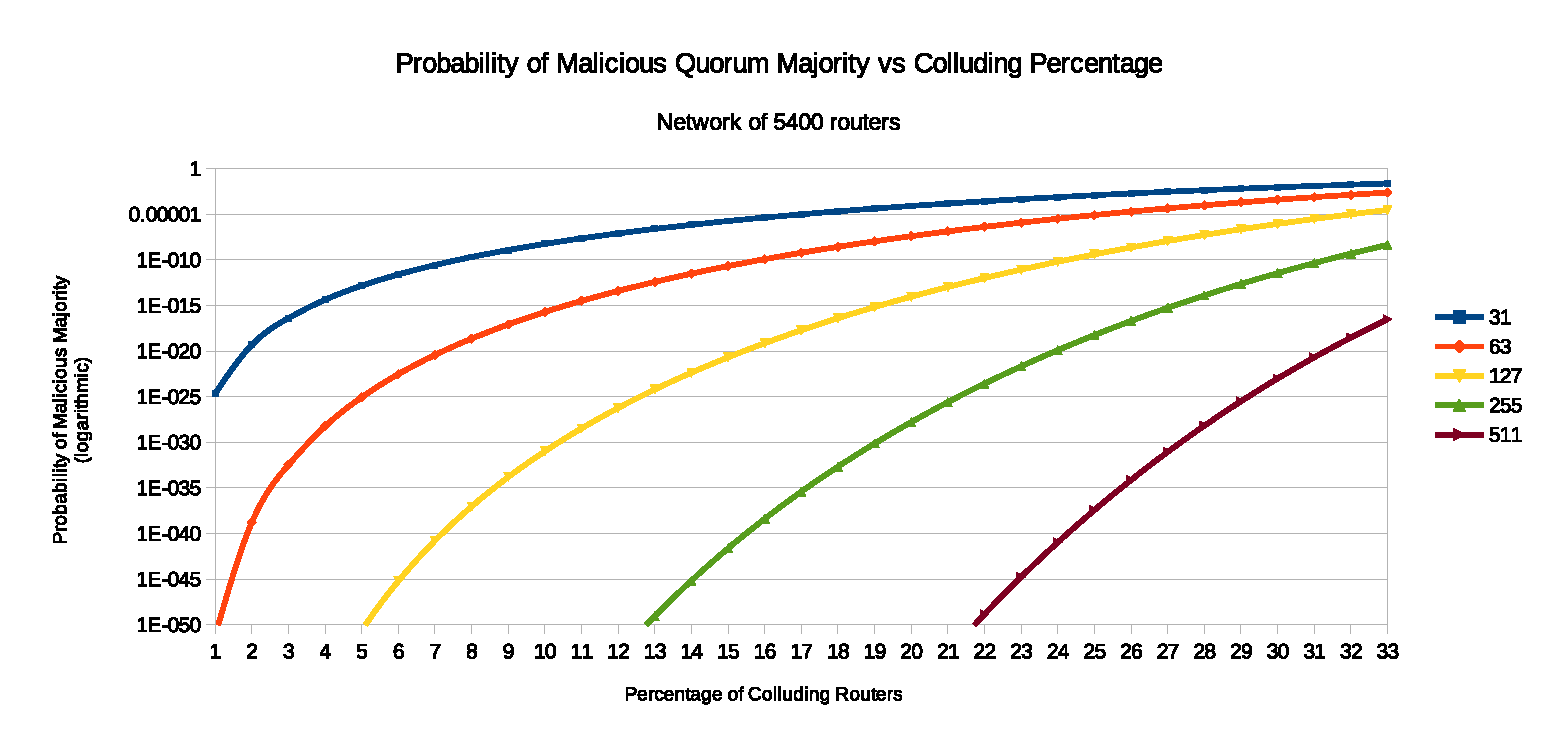
\includegraphics[width=0.5\textwidth]{../analysis/MaliciousQuorumProbability.eps}
%	\caption{The probability that Eve controls the majority of the Quorum is given by the PMF of the hypergeometric distribution. We fix $ N $ at 5,400 nodes and graph Eve's success probability as a function of an increasing percentage of Eve-controlled colluding routers. We examine five selections for $ L_{Q} $: 31, 63, 127, 255, and 511. We do not consider percentages beyond 33 percent as 33 percent represents a complete compromise of the Tor network: it is near 100 percent that the three routers selected during circuit construction are under Eve's control, a violation of our security assumptions.}
%	\label{chart:quorumMajority}
%\end{figure}
%
%Figure \ref{chart:quorumMajority} shows that a choice of $ L_{Q} = 31 $ is suboptimal: the probabilities are above the $ 10^{-38.532} $ threshold for even small levels of collusion. $ L_{Q} = 63 $ likewise fails with approximately two percent collusion, although choices of 127, 255, and 511 fail at levels above approximately 8, 16, and 25 percent, respectively. The figure also suggests that larger Quorums are superior with respect to security. Small Quorums are also less resilient to DDOS attacks at the Quorum in general.
%
%If we assume that Eve controls 10 percent of the Tor network, then we can examine the impact of the longevities of Quorums; over a fixed period of time, slower rotations suggests a lower cumulative chance of selecting any malicious Quorum. If $ w $ is Eve's chance of compromise, then her cumulative chances of compromising any Quorum is given by $ 1 - (1-2)^t $. This gives us a bound estimate on $ \Delta q $. We estimate this over 10 years in Figure \ref{chart:cumulativeProbability}.
%
%\begin{figure}[htbp]
%	\centering
%	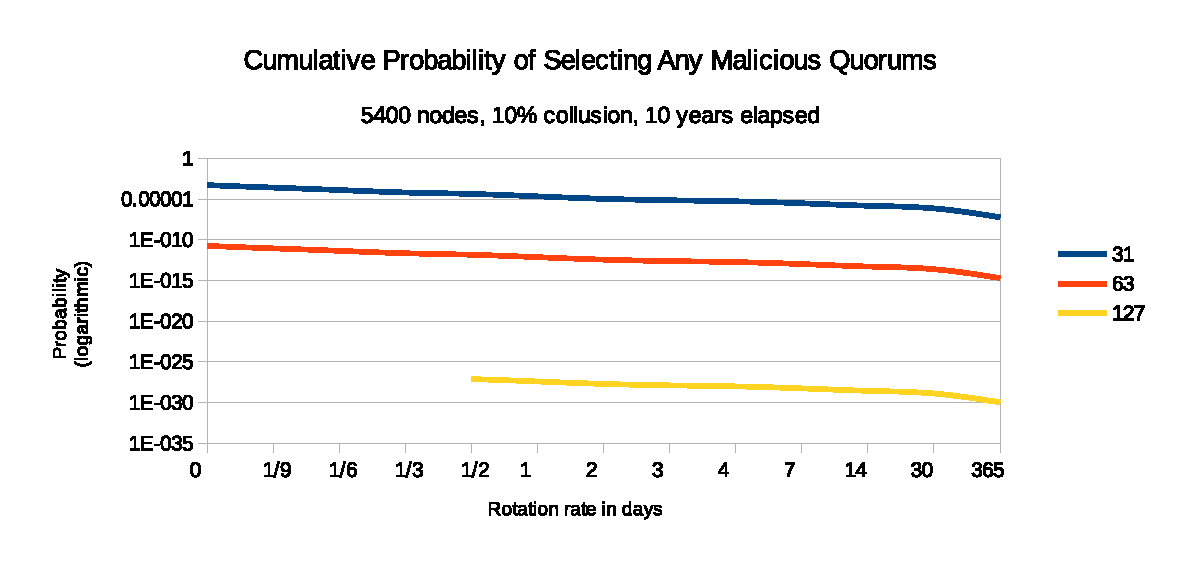
\includegraphics[width=0.5\textwidth]{../analysis/CumulativeMaliciousQuorum.eps}
%	\caption{The cumulative probability that Eve controls any Quorum at different rotation rates. We assume 10 percent collusion in a network of 5400 Tor routers, and view across 10 years. We do not graph $ L_{Q} $ values of 255 or 511 as they generate probabilities far below our $ 10^{-38.532} $ threshold; $ L_{Q} = 255 $ and $ L_{Q} = 511 $ produce values less than $ 10^{-58} $ and $ 10^{-134} $, respectively.}
%	\label{chart:cumulativeProbability}
%\end{figure}
%
%Figure \ref{chart:cumulativeProbability} suggests that while slow rotations (i.e a period of 7 days) generates orders of magnitude less chance than fast rotations, the choice of $ L_{Q} $ is far more significant. Like Figure \ref{chart:quorumMajority}, it also shows that $ L_{Q} = 31 $ and $ L_{Q} = 61 $ are relatively poor choices.
%
%If a selected Quorum is malicious, fast rotation rates will minimize the duration of any disruptions, as shown in Figure \ref{chart:quorumLongevity}. This figure suggests that fast rotations are optimal in that respect, a contradiction to Figure \ref{chart:quorumMajority}. However, given the very low statistical likelihood of selecting a malicious Quorum, we consider this a minor contribution to the decision.
%
%Although a malicious Quorum would have the capabilities to deploy a variety of attacks on the network, the proper selections of $ L_{Q} \geq 127 $ and $ \Delta q \geq 1 $ reduces the likelihood of this occurring to near-zero probabilities. We consider this a stronger solution than introducing countermeasures to those attacks. Based on our security analysis, we suggest $ L_{Q} \geq 127 $ and $ \Delta q \geq 1 $. However, the networking and performance load scales linearly with Quorum size. Based on this balance and our above analysis, we suggest 127 or 255 for values of $ L_{Q} $ and 7 or 14 for $ \Delta q $.
%
%\subsection{Entropy of Tor Consensus Documents}
%
%We use Tor's consensus documents as a sources of entropy agreed upon by all parties, however we have not yet demonstrated that the network status contains enough entropy to provide reasonable assurance that Eve cannot guess the next Quorum in advance. If Eve could predict future Quorums, Eve can subvert the Quorum Derivation protocol in a variety of attack vectors. However, this would fail our security assumption against adaptive compromise in the presence of OnioNS. Rather than introducing defences against these attack vectors, we nevertheless believe that ensuring sufficient entropy in the consensus documents is a superior defence.
%
%%	\item \textbf{dir-source:} The authority's nickname, fingerprint, IP address, onion routing port, and directory port.
%%	\item \textbf{contact:} Optional contact information for the authority operator.
%%	\item \textbf{vote-digest:} The hash of the authority's status vote document.
%%	
%%	\item \textbf{r:} The router's nickname, fingerprint, time of last restart, IP address, onion routing port, and directory port.
%%	\item \textbf{m:} The SHA-256 hash of the router's microdescriptor. This also includes its entries in the \emph{cached-microdescs} document (discussed below).
%%	\item \textbf{s:} A list of the router's status flags, as given by the directory authorities. Common examples include Running, Valid, Fast, Guard, Stable, and Exit.
%%	\item \textbf{v:} The version of the Tor software that the router is running, as reported by the router.
%%	\item \textbf{w:} The estimated bandwidth that this router is capable of. This value is determined by speed tests from bandwidth authorities, who are a subset of the directory authorities.
%
%In section \ref{sec:ConsensusDocs} we detailed the significant contents of the three consensus documents relevant to OnioNS, \emph{cached-certs}, \emph{cached-microdesc-consensus}, and \emph{cached-microdescs}. As we stated in section \ref{sec:Protocols}, the Quorum Derivation protocol only utilizes the \emph{cached-certs} and \emph{cached-microdesc-consensus} documents for reasons we discuss below.
%
%\subsubsection{cached-certs}
%
%The \emph{cached-certs} document contains long-term directory identity keys and medium-term signing keys. While Eve cannot predict the public half of new signing keys in advance, the keys rotate every 3-12 months\cite{TorDirSpec} so \emph{cached-certs} is not a timely source of entropy. Nevertheless, if an attacker can predict the network status described in \emph{cached-microdesc-consensus}, the rotation timeline of the signing keys in \emph{cached-certs} places an absolute upper-bound on the duration of Quorum predictability.
%
%\subsubsection{cached-microdesc-consensus}
%
%The \emph{cached-microdesc-consensus} document describes the network status and is our main source of entropy. In the header, the  \emph{vote-digest} header is the hash of a directory authority's status vote. Each directory operates independently and there are nine directory authorities, so we consider this value unpredictable. Router descriptors follow the header in the body of the document. 
%
%The $ r $ field in a router's descriptor contains routing information and time of last restart. Tor routers have no guarantee of availability and routers may restart for a variety of reasons. As of April 2015 Tor's network consists of approximately 7,000 routers \cite{TorMetrics} and assuming that a given router restarts every 60 days, statistically the number of unpredictable $ \emph{r} $ fields each day is given by $ \frac{7000}{60} \approx 116.66 $. Tor displays the restart time down to the second, so each restart adds approximately six bytes of entropy, for an estimated total of $ \frac{7000 * 6}{60} = 700 $ bytes of short-term entropy from the $ r $ field.
%
%%The $ s $ field contains a list of flags given to the router by the directory authorities according to qualification rules. $ s $ is thus predictable if an attacker can monitor the descriptor
%
%The $ v $ field describes the version of Tor that the router is running. Although the versions of Tor are publicly known and the official and unofficial Linux repositories are publicly accessible, Eve cannot predict when an administrator will upgrade their router to the next available Tor version. Although new versions of Tor are not frequently released and routers are upgraded infrequently as shown in Figure \ref{fig:TorVersions}, the $ v $ field still introduces a degree of medium-term entropy into the document.
%
%The $ w $ field contains the router's estimated bandwidth capacity as calculated by bandwidth authorities. Clients use this field during circuit construction; routers with a higher bandwidth capacity relative to the rest of the network have a higher probability of being included in a circuit. Although it is likely that a given router will have similar bandwidth measurements between consecutive consensus documents, Eve cannot predict the exact performance of a router from the perspective of the bandwidth authority. Eve's capacity to predict the performance of all routers falls outside of Tor's and OnioNS' security assumptions; Eve must therefore be a global attacker who would be capable of compromising the Tor network as a whole anyway.
%
%We note that significant amounts of additional entropy could be trivially added into \emph{cached-microdesc-consensus} if each router added a single random byte to their descriptor or if the directory authorities each contributed entropy.
%
%\subsubsection{cached-microdescs}
%
%Although we did not detail it in section \cite{TorDirSpec}, in practice Tor places client-side timestamps inside \emph{cached-microdescs}. These timestamps would significantly divide the network, causing \emph{cached-microdescs} to be ill-suited for inclusion in the Quorum Derivation protocol. Although \emph{cached-microdescs} contains long-term router keys and the fingerprints of routers in the same family which would both serve as a source of long-term entropy, \emph{cached-microdesc-consensus} contains the SHA-256 hashes of the router descriptor. We therefore do not include it when hashing the documents in the Quorum Derivation protocol.
%
%\subsection{Malicious Entropy Reduction}
%
%The Quorum Derivation protocol describes initializing the Mersenne Twister with a 384-bit seed. If we assume that Eve desires that the Quorum Derivation protocol produce a Quorum pleasing to Eve (such as including her malicious routers in the Quorum or rejecting specific honest routers from the Quorum) then Eve can find $ k $ seeds that generates a desirable scrambled list in $ 2^{192} $ operations on average, or $ 2^{384} $ operations in the worst case. The chance of any of those seeds being selected is $ \frac{2^{384}}{k} $. 
%
%If we also assume that Eve can predict some fraction $ f \in {(0, 1)} $ of the contents of the consensus documents, then Eve may attempt to manipulate her router's descriptors such that the Quorum Derivation protocol produces one of the $ k $ hashes. SHA-384's strong resistance to preimage and second preimage attacks requires $ 2^{192} $ operations on average for Eve to find one of the $ k $ hashes. This difficulty is compounded by the limited combinatorics within the set of valid router descriptors. The number of operations involved in this attack vector is significantly more than the operations involved in breaking AES, so we disregard the possibility of manipulating the Quorum Derivation protocol in this way. We do not consider the possibility of Eve controlling the entire consensus document, this would severely compromise the integrity of the Tor network and thus violates our security assumptions.
%
%\subsection{Sybil Attacks}
%
%Eve may also attempt to increase her probability of including her malicious nodes in the Quorum via Sybil attacks. We offer no defence against this type of attack, although Tor does. The attack is difficult to carry out in practice due to the slow build of trust within the Tor network. Directory authorities would give Eve's nodes the Fast and Stable flags after weeks of continual uptime and a history of reliability. For large-scale Sybil attacks, this introduces a significant time and financial cost to Eve. We also note that choices of $ L_{Q} $ and $ \Delta q $ also offer significant statistical defences against Sybil attacks, as illustrated in Figures  \ref{chart:quorumMajority} and \ref{chart:cumulativeProbability}, shown above.
%
%\subsection{Hidden Service Spoofing}
%
%OnioNS does not require a hidden service operator to reveal any personally-identifiable information. Hidden services are only known by their public key and domain names, and we assume that the hidden service is authentic. We have also observed spoofed hidden services in the wild, suggesting that this problem already exists in Tor's environment. We do not introduce a reputation system or distributed verification system, and note that it is difficult if not impossible to construct a reliable defence against hidden service spoofing attacks due to their anonymous nature. 
%
%One possible solution, although it severely compromises anonymity, is to register a hidden service with an SSL Certificate Authority and apply an SSL certificate to the server. In this way, TLS communication provides an authenticity check against the hidden service, although TLS also sets up a redundant encryption layer that may decrease performance. However, in practice this solution is very rarely seen; out of approximately 25,000 hidden services,\cite{TorMetrics}\cite{kadianakis2015extrapolating} to date only three hidden services have browser-trusted SSL certificates: Blockchain.info at https://blockchainbdgpzk.onion, Facebook at https://facebookcorewwwi.onion, and The Intercept's SecureDrop instance at https://y6xjgkgwj47us5ca.onion. In future work we may study the security implications of signing the .onion address or the .tor OnioNS domain name. Due to their severe privacy concerns and the security controversy surrounding the centralized CA Chain of Trust, generally speaking we do not recommend the application of SSL certificates to Tor hidden services. 
%
%\subsection{Outsourcing Record Proof-of-Work}
%
%%Scrypt introduces a cost and its memory demands increases the difficulty of custom hardware and massively-parallel attacks, effectively limiting adversaries to the same hardware as legitimate users.
%
%The Record Generation protocol can safely take place within an offline machine under the operator's control. We designed the Record Generation protocol with the objective of requiring the hidden service operator to also perform the scrypt proof-of-work. However, our protocol does not entirely prevent the operator from outsourcing the computation to secondary resource in all cases.
%
%Let Bob be the hidden service operator, and let Craig be a secondary computational resource. We assume that Craig does not have Bob's private key. Then,
%
%\begin{enumerate}[noitemsep,nolistsep]
%	\item Bob creates an initial Record $ R $ and completes the \emph{type}, \emph{nameList}, \emph{contact}, \emph{timestamp}, and \emph{consensusHash} fields.
%	\item Bob sends $ R $ to Craig.
%	\item Let $ \mathit{central} $ be $\mathit{type} \concat \mathit{nameList} \concat \mathit{contact} \concat \mathit{timestamp} \concat \mathit{consensusHash} \concat \mathit{nonce} $.
%	\item Craig generates a random integer $ K $ and then for each iteration $ j $ from 0 to $ K $,
%		\begin{enumerate}[noitemsep,nolistsep]
%			\item Craig increments \emph{nonce}.
%			\item Craig sets \emph{PoW} as $ \mathrm{PoW}(\mathit{central}) $.
%			\item Craig saves the new $ R $ as $ C_{j} $.
%		\end{enumerate}
%	\item Craig sends all $ C_{0 \le j \le K} $ to Bob.
%	\item For each Record $ C_{0 \le j \le K} $ Bob computes
%		\begin{enumerate}[noitemsep,nolistsep]
%			\item Bob sets \emph{pubHSKey} to his public RSA key.
%			\item Bob sets \emph{recordSig} to $ S_{d}(m, r) $ where $ m = \mathit{central} \concat \mathit{pow} $ and $ r $ is Bob's private RSA key.
%			\item Bob has found a valid record if $ H(\mathit{central} \concat \mathit{pow} \concat \mathit{recordSig}) \leq 2^{\mathit{difficulty} * \mathit{count}} $
%		\end{enumerate}
%\end{enumerate}
%
%% todo: calculate chances of Craig computing a correct record
%
%Our protocol ensures that Craig must always compute more scrypt iterations than necessary; Craig cannot generate \emph{recordSig} and thus cannot compute if the hash is below the threshold. Moreover, the scrypt work incurs a cost onto Craig that must be compensated financially by Bob. Thus the Record Generation protocol places a lower bound on the cost paid by Bob.
%
%%\subsection{False Negatives Claims}
%%
%%OnionNS records are self-signed and include the hidden service's public key, so anyone --- particularly the client --- can confirm the authenticity (relative to the authenticity of the public key) and integrity of any record. This does not entirely prevent Sybil attacks, but this is a very hard problem to address in a distributed environment without the confirmation from a central authority. However, the proof-of-work component makes record spoofing a costly endeavour, but it is not impossible to a well-resourced attacker with sufficient access to high-end general-purpose hardware.
%%
%%Hidden service .onion addresses will continue to have an extremely high chance of being securely unique as long the key-space is sufficiently large to avoid hash collisions.
%%
%%As we have stated earlier, falsely claiming a negative on the existence of a record is a problem overlooked in other domain name systems. One of the primary challenges with this approach is that the space of possible names so vast that attempting to enumerate and digitally sign all names that are not taken is highly impractical. Without a solution, this weakness can degenerate into a denial-of-service attack if the DNS resolver is malicious towards the client. Our counter-measure is the highly compact hashtable bitset with a Merkle tree for collisions. We set the size of the hashtable such that the number of collisions is statistically very small, allowing an efficient lookup in $ \mathcal{O}(1) $ time on average with minimal data transferred to the client.
%
%\subsection{DNS Leakage}
%
%Human mistakes can also compromise user privacy. One such security threat is the accidental leakage of .tor lookups over the Internet DNS. This vulnerability is not limited to OnioNS and applies to any alternative DNS; users may mistakenly attempt lookups over the traditional Internet DNS. Mohaisen and Thomas observed .onion lookups on root DNS servers at a frequency that corresponded to external global events, highlighting the human factor in those leakages.\cite{thomasmeasuring} For OnioNS, this may occur if their client software was not properly configured, if their browser was not properly configured to or could not communicate with Tor, or for other reasons. We offer no defence against this attack vector and note that any defence against it would need to introduce lookup whitelists or blacklists into common browsers such as Chrome, Firefox, and Internet Explorer to prevent them from attempting lookups for pseudo-TLDs.
%
%%\section{Reliability}
%
%%\subsubsection{Flooding}
%
%%\emph{What happens if Quorum nodes are unavailable? How is their unavailability secured for future reference? What are the implications of a Quorum node withholding or forging a Record before flooding their Snapshot out? Can a single node mislead the rest of the Quorum?}
%
%%Although this approach does not entirely thwart Sybil attack, this attack vector is difficulty to impossible to counter in a privacy-enhanced environment, and trading anonymity for defence is highly undesirable.
%
%%\emph{Tor nodes provide no guarantee of availability. What are the implications of Quorum nodes or Mirrors suddenly disappearing? How can data be lost? What if a Quorum node is offline temporarily during active duty, will it catch up?}
%
%%  on Unreliable Hosts
%
%%Tor nodes have no reliability guarantee and may disappear from the network momentarily or permanently at any time. Old \emph{quorums} may disappear from the network without consequence of data loss, as their data is cloned by current \emph{mirrors}. So long as the \emph{quorum} nodes remain up for the $ \Delta i $ days that they are active, the system will suffer no loss of functionality. Nodes that become temporarily unavailable will have out-of-sync \emph{pages} and will have to fetch recent records from other \emph{quorum} nodes in the time of their absence.
%
%\section{Objectives Assessment}
%
%OnioNS achieves all of our original requirements:
%
%\begin{enumerate}[noitemsep,nolistsep]
%	\item \textbf{The system must support anonymous registrations} --- OnioNS Records do not contain any personal or location information. The PGP key field is optional and may be provided if the hidden service operator wishes to allow others to contact him. However, the operator may be using an email address and a Web of Trust disassociated from his real identity, in which case no identifiable information is exposed.
%	\item \textbf{The system must support privacy-enhanced lookups} --- OnioNS performs Domain and Onion Queries through Tor circuits, and under our original assumption that circuits provide strong guarentees of client privacy and anonymity, resolvers cannot sufficiently distinguish users to track their lookups.
%	\item \textbf{Clients must be able to authenticate registrations} --- OnioNS Records are self-signed, enabling Tor clients to verify the digital signature on the domain names and check the public key against the server's key during the hidden service protocol. This ensures that the association has not been modified in transit and that the domain name is authentic relative to the authenticity of the destination server.
%	\item \textbf{Domain names must be provably or have a near-certain chance of being unique} --- Tor hidden services .onion addresses are cryptographically generated with a key-space of $ 58 ^ {16} \approx 2 ^ {93.727695922} $ and domain names within OnioNS are provably unique by anyone holding a complete copy of the Pagechain.
%	\item \textbf{The system must be distributed} --- The responsibilities of OnioNS are spread out across many nodes in the Tor network, decreasing the load and attack potential for any single node. The Pagechain is likewise distributed and locally-checked by all Mirrors, and although its head is managed by the Quorum, these authoritative nodes have temporary lifetimes and are randomly selected. Moreover, Quorum nodes do not answer queries, so they have limited power.
%	\item \textbf{The system must be simple and relatively easy to use} --- Domain Queries are automatically resolved and require no input by the user. From the user's perspective, they are taken directly from a meaningful domain name to a hidden service. Users no longer have to use unwieldy .onion addresses or review third-party directories, OnioNS introduces memorability to hidden service domains.
%	\item \textbf{The system must be backwards compatible with existing protocols} --- OnioNS does not require any changes to the hidden service protocol and existing .onion addresses remain fully functional. Our only significant change to Tor's infrastructure is the mechanism for distributing hashes for the Quorum Qualification protocol, but our initial technique for using the Contact field minimizes any impact. We also hook into Tor's TLD checks, but this change is very minor. Our reference implementation is provided as a software package separate from Tor per the Unix convention.
%\end{enumerate}
%
%Finally, we meet our optional performance objectives:
%
%\begin{enumerate}[noitemsep,nolistsep]
%	\item \textbf{The system should not require clients to download the entire database} --- Only Mirrors hold the Pagechain, and clients do not need to obtain it themselves to issue a Domain Query. Therefore clients rely on their existing and well-established trust of Tor routers when resolving domain names. However, clients may optionally obtain the Pagechain and post Domain Queries to localhost for greater privacy and security guarantees.
%	\item \textbf{The system should not introduce significant burdens to the clients} --- Record verification should occur in sub-second constant time in most environments, and Ed25519 achieves very fast signature confirmation so verifying Page signatures at level 1+ takes trivial time. However, clients also verify the Record's proof-of-work, so for some scrypt parameters the client may spend non-trivial CPU time and RAM usage confirming the one scrypt iteration required to check. We must therefore choose our parameters carefully to reduce this burden especially on low-end hardware.
%	\item \textbf{The system should have low latency} --- Domain Queries without any packet delays over Tor low-latency circuits. Its exact performance is largely dependent on circuit speed and the client's verification speed.
%\end{enumerate}
%
%We therefore believe that we have squared Zooko's Triangle; OnioNS is distributed, enables hidden service operators to select human-meaningful domain names, and domain names are guaranteed unique by all participants.
%
%\section{Future Work}
%
%In future work we will expand our implementation of OnioNS and develop the remaining protocols. While our implementation functions with a fixed resolver, we will deploy our implementation onto larger and more realistic simulation environments such as Chutney and PlanetLab. When we have completed dynamic functionality and the remaining protocols, we will pursuit integrating our implementation into Tor. We expect this to be straightforward as OnioNS is designed as a plugin for Tor, introduces no changes to Tor's hidden service protocol, and requires very few changes to Tor's software. In future developments, Tor's developers may also make significant changes to Tor's hidden services, but OnioNS' design enables our system to become forwards-compatible after a few minor changes.
%
%Additionally, several questions need to answered in future studies:
%
%\begin{itemize}[noitemsep,nolistsep]
%	\item Should the Quorum expire registrations that point to non-existent hidden services, and if so, how can this be done securely?
%	\item How can we reduce vulnerability to phishing/spoofing attacks? Can OnioNS be adapted to include a privacy-enhanced reputation system?
%	\item How can OnioNS support domain names with international encodings? A na\"{i}ve approach to this is to simply support UTF-16, though care must also be taken to prevent phishing attacks by domain names that use Unicode characters that visually appear very similar.
%	\item What other networks can OnioNS apply to? We require a fully-connected networked and an global source of entropy. We encourage the community to adapt our work to other systems that fit these requirements.
%\end{itemize}
%
%\section{Reference Implementation}
%
%Alongside this publication, we provide a reference implementation of OnioNS. We utilize C++11, the Botan cryptographic library, the Standard Template Library's (STL) implementation of Mersenne Twister, and the libjsoncpp-dev library for JSON encoding. We develop in Linux Mint and compile for Ubuntu Vivid, Utopic, Trusty, and their derivatives. Our software is built on Canonical's Launchpad online build system and is available online at \url{https://github.com/Jesse-V/OnioNS}. 
%
%\subsection{Prototype Design}
%
%We have developed an OnioNS prototype that implements the Domain Query protocol. In this initial prototype, we use a static server, a single fixed Create Record, and a hidden service that we deployed at onions55e7yam27n.onion. Although our implementation is primarily a separate software package, we made necessary modifications to the Tor client software to intercept the .tor pseudo-TLD, pass the domain to the OnioNS client over inter-process communication (IPC), and receive and lookup the returned hidden service address. We diagram the relationships between our prototype's components in Figure \ref{fig:prototypeDiagram}.
%
%Our prototype's works as follows:
%
%\begin{enumerate}[noitemsep,nolistsep]
%	\item The user enters in ``example.tor'' into the Tor Browser.
%	\item The Tor Browser sends ``example.tor'' to Tor's SOCKS port for resolution.
%	\item The Tor client intercepts ``*.tor'', places the lookup in a wait state, and sends ``example.tor'' to the OnioNS client over a named pipe.
%	\item The OnioNS client communicates with Tor's SOCKS port and negotiates a connection to the static OnioNS server.
%	\item The OnioNS client performs a level 0 Domain Query to the server.
%	\item The server responds with the Create Record containing ``example.tor''.
%	\item The client writes ``onions55e7yam27n.onion'' to the Tor client over another named pipe.
%	\item The Tor client resumes the lookup and overrides the original ``example.tor'' lookup with ``onions55e7yam27n.onion''.
%	\item The Tor client contacts the OnioNS hidden service and passes the webpage to the Tor Browser.
%	\item The Tor Browser displays the website contents and preserves the ``example.tor'' domain name.
%\end{enumerate}
%
%\subsection{Performance}
%
%We created a rudimentary form of the Record Generation and Client Verification protocols and conducted performance measurements on two different machines. We tested these protocols on Machine A, which has an Intel Core2 Quad Q9000 @ 2.00 GHz; and machine B, which has an Intel i7-2600K @ 4.3 GHz. We chose machines with this hardware in order to more accurately determine the performance with out target audience; Machines A and B represent low-end and medium-end consumer-grade computers, respectively. To minimize latency on our end, both machines were hosted on 1 Gbits connections at Utah State University. As the Record Generation protocol requires a hidden service private key, we created a hidden service and hosted it on Machine B, using Shallot, a vanity key generator, to generate a recognizable hidden service address, \url{http://onions55e7yam27n.onion}. Then on Machine A, we measured the time required to connect to our hidden service over OnioNS and over the more direct hidden service protocol.
%
%We selected the parameters of scrypt such that it consumed 128 MB of RAM during operation. This is an affordable amount of RAM by even low-end consumer-grade machines. This RAM consumption scales linearly with the number of scrypt instances executed in parallel. We used all eight cores on Machine B to generate a Record for our hidden service and observed approximately 1 GB of RAM consumption, matching our expectations. We set the difficulty of the Create Record such that the Record Generation protocol took only a few minutes on average to conduct, but in the future we may change it so that the protocol takes several hours instead.
%
%\subsubsection{Processing Time}
%
%We measured the CPU wall time required for different parts of client-side protocols. We measured how long it takes the client to build a Record from a JSON-formatted textual string, which involves parsing and assembly of the various fields; the time to check the proof-of-work \emph{PoW}, and the time to check the \emph{recordSig} digital signature.
%
%\renewcommand{\arraystretch}{1}
%\begin{center}
%    \begin{tabular}{ | c | c | c | c |}
%    \hline
%    \textbf{Description} & \textbf{A Time (ms)} & \textbf{B Time (ms)} & \textbf{Samples} \\
%    \hline
%    Parsing JSON into a Record & 0.052 & 0.0238 & 100 \\ \hline
%	Scrypt check & 896.369 & 589.926 & 25 \\ \hline
%	Check of $ S_{d}(m, r) $ RSA signature & 0.06304 & 0.0267 & 200 \\
%	\hline
%    \end{tabular}
%\end{center}
%
%Machine B, as expected, performed much faster than Machine A at all of these tasks. Parsing and signature checks both took trivial time, though the total time was dominated by the single iteration of scrypt. Record Validation protocol is single threaded and consumes 128 MB of RAM due to scrypt.
%
%\subsubsection{Latency}
%
%We compared the load latency between an OnioNS domain name with a traditional hidden service address. Our tests measured the time between when a user entered in ``example.tor'' into the Tor Browser to the time when the browser first began to load our hidden service webpage. We also tested \url{http://onions55e7yam27n.onion}, the destination of ``example.tor''. We performed our experiment 15 times with a different client-side Tor circuit for each by restarting Tor at each iteration. To prevent browser-side caching, we restarted the Tor Browser between tests as well. 
%
%\renewcommand{\arraystretch}{1}
%\begin{center}
%    \begin{tabular}{ | c | c | c | c |}
%    \hline
%    \textbf{Lookup} & \textbf{Fastest Time} & \textbf{Slowest Time} & \textbf{Mean Time} \\
%    \hline
%    .tor & 6.1 & 8.5 & 7.1 \\ \hline
%	.onion & 9.3 & 12.2 & 10.2 \\
%	\hline
%    \end{tabular}
%\end{center}
%
%The latency is circuit-dependent and heavily depends on the speed of each Tor router and the distance between them. To avoid the latency cost whenever possible, we implemented a DNS cache into the OnioNS client-side software to allow subsequent queries to be resolved locally, avoiding unnecessary remote lookups.
%
%\subsection{Future Work}
%
%We have several plans for future work. First, we will port the OnioNS client to Windows and migrate the Tor-OnioNS IPC from Unix named pipes to TCP sockets. Although named pipes work reliably in Unix-like operating systems, they are not easily compatible in the Windows family of operating systems. Second, we will find more optimal parameters for scrypt to increase performance and work to reduce the latency. Finally, we will expand our implementation and collaborate with Tor developers to merge it into Tor's repositories when it is complete.
%
%\section{Conclusion}
%
%We have introduced OnioNS, a Tor-powered distributed DNS that maps unique .tor domain names to traditional Tor .onion addresses. It enables hidden service operators to select a human-meaningful domain name and provide access to their service through that domain. We preserve the privacy and anonymity of both parties during registration, maintenance, and lookup, and furthermore allow Tor clients to verify the authenticity of domain names. Moreover, we rely heavily upon existing Tor infrastructure, which simplifies our design assumptions and narrows our threat model largely to attack vectors already well-understood throughout the Tor literature.
%
%We use the Pagechain distributed data structure to prevent disagreements from forming within the network. Furthermore, every participant can verify the uniqueness of domain names. The Pagechain also has a fixed maximal length, which places an upper bound on the networking, computational, and storage requirements for all participants, a valuable efficiency gain especially noticeable long-term.
%
%OnioNS achieves all three properties of Zooko's Triangle: it is distributed, allows hidden service operators to select meaningful domain names, and all parties can confirm for themselves the uniqueness of domain names in the database. We provide a reference implementation in C++ that should enable Tor developers to deploy OnioNS into the Tor network with minimal effort. We believe that OnioNS will be a useful abstraction layer that will significantly enhance the usability and the popularity of Tor hidden services.
%
%\section{Acknowledgements}
%
%We would also like to thank Tor developers Mark Ellzey, Yawning Angel, and Nick Mathewson for their assistance with libevent and Tor technical support and Sarbajit Mukherjee for his commentary.

\bibliographystyle{abbrv}
\bibliography{citations}

\end{document}
